% master.tex : master file for the project
% ------------------------------------------------------------------------------
% This is the main file in the project, which collects the contents from all the
% input files (text, images, literature databases, etc.).

% The 'book' class is a document class with many flexible options.
% See https://tex.stackexchange.com/a/36989/118167
\documentclass[11pt,a4paper,twoside,openright,english]{book}
 
% Some top level variables that are used to automatically input title, authors,
% etc. in the title page and front page.
\def \projecttitle       {Advanced Topics with Applications}
\def \projectsubtitle    {Pricing under Rough Volatility}
\def \projecttheme       {Project Theme}
\def \projectdegree      {Mathematics-Economics}  % or Mathematics-Economics/Technology
\def \projectperiod      {Autumn Semester 2023}
\def \projectnumber      {P9}
\def \projectgroup       {X}
\def \projectauthors     {
  Christian Bang Jensen \\
  % ...
}
\def \projectsupervisors {
  Orimar Sauri\\
  % ...
}

% The preamble, i.e. all the settings and commands that go before actual
% document contents, in this template is handled in the single file aaumath.sty,
% which defines a package that can be loaded here with \usepackage.
\usepackage{aaumath}
\usepackage{soul}
% All contents of the document go between the \begin and \end commands for the
% 'document' environment.
\begin{document}

% The front matter is not counted in the numbered pages and are instead numbered
% with roman numerals. This consists of, for example, the front page, title
% page, preface, and table of contents.
\frontmatter
% incl/misc/frontpage.tex : document front page
% ------------------------------------------------------------------------------


\backgroundsetup{
  scale = 1,
  angle=0,
  opacity=1,
  contents = {
    
\includegraphics[width=\paperwidth,height=\paperheight]{fig/img/aau/waves.pdf}
  }
}
\BgThispage
\pdfbookmark[0]{Front page}{frontpage}
\begin{titlepage}
  \centering
  \phantom{}
  \vspace{2cm}

  % AAU badge
  \begin{minipage}[c]{0.2\paperwidth}
    \centering
    \makebox[0pt]{
      % fig/tikz/aau-badge.tex : AAU logo badge for the front page
% ------------------------------------------------------------------------------

\begin{tikzpicture}
  % Draw white circle and add the transparent blue logo on top
  \node[circle,color=white,fill=white,minimum size=1.175\textwidth] at (0,0) {};
  \node at (0,0) {
\includegraphics[width=\textwidth]{fig/img/aau/logo-circle.pdf}};
\end{tikzpicture}

    }
  \end{minipage}

  % Main contents
  \vspace{4cm}
  {\fontfamily{bch}\selectfont
    \fboxsep0pt\colorbox{white}{
      \begin{minipage}{\textwidth}
        \centering
        \color{AAUblue1}

        \vspace{2em}
        {\Huge\bfseries\projecttitle}
        {\Large\bfseries\projectsubtitle}

        \bigskip
        \parbox{\textwidth}{\centering\large\projectauthors}

        \bigskip
        {\bfseries\large{\projectnumber} Project, Group \projectgroup, \projectdegree}
        \vspace{2em}
      \end{minipage}
    }
  }

\end{titlepage}

% incl/misc/titlepage.tex : project title page
% ------------------------------------------------------------------------------
% The title page is generated by the command \aautitlepage, which is defined in
% /incl/pre/ext/aautitlepage.sty


\pdfbookmark[0]{Title page}{titlepage}
\aautitlepage{
  \projectinfo{
    Advanced Topics with Applications
  }{
    Pricing under Rough Volatility
  }{
    Autumn Semester 2023
  }{
    Group 1.204f
  }{
    Christian Bang Jensen
  }{
    \parbox[t]{\textwidth}{Orimar Sauri\\
    Toke Zinn}
  }{
    \today
  }
}{
  \textbf{Dept. of Mathematical Sciences}\\
  Skjernvej 4A\\
  DK-9220 Aalborg Ø\\
  \href{http://math.aau.dk}{http://math.aau.dk}
}{
  % incl/misc/abstract.tex : project abstract
% ------------------------------------------------------------------------------
% The abstract is a short summary of the document, displayed on the title page
So if you like see a point that is like different then like don't. 

%We find a model which determines the number of deaths due to COVID-19 based on several factors in different countries and then we test which of these factors that does in fact influence the number of deaths. }
\section*{Preface}
\addcontentsline{toc}{chapter}{\protect\numberline{}Preface}
%This project report is written as a 4th semester project during the spring semester of 2020 as part of the programme in Mathematics-Economics at the Department of Mathematical Sciences at Aalborg University. The overall topic of the report is \textit{Mathematical Modelling in Finance} with a focus on how expected utility theory can be used in the insurance markets.  

%The project is composed of numbered chapters with corresponding sections and subsections. Citations and external references are made using the Vancouver system such that \cite[p.~10]{axler} refers to page 10 of the first entry in the bibliography. All programming is performed using R, and the R-code can be found in the appendices at the end of the report. 

This project report is written as a 6th semester project during the spring semester of 2021 as part of the programme in Mathematics-Economics at the Department of Mathematical Sciences at Aalborg University. 

%The overall topic of the report is \textit{Statistical Modelling and Analysis} with a focus on how statical theory and data analysis can be utilized to determine the comorbidities of COVID-19.


The project is composed of numbered chapters with corresponding sections and subsections. Citations and external references are made using the Vancouver system such that xx refers to page 10 of the first entry in the bibliography. All programming is performed using R, and the R-code can be found  at the following GitHub repository: 


Finally, the group would like to extend our appreciation to our supervisor Sauri Arregui Orimar. 
\bigskip
\subsection*{Signatures}
\begin{tabular}{lcl}
    & &\\
    & &\\
    \rule{7cm}{1pt} & \hspace{0.5cm} & \rule{7cm}{1pt} \\
    \vspace{1.5cm}
    Christian Bang Jensen & & Houssam Al-Hanafi \\
    \rule{7cm}{1pt} & \hspace{0.5cm} & \rule{7cm}{1pt} \\
    \vspace{1.5cm}
    Rasmus Nørrevang & & Sebastian Søndergaard Kure\\
    \rule{7cm}{1pt} & \hspace{0.5cm} & \\
    \vspace{1.5cm}
    Søren Thode 
\end{tabular}
\vspace{1cm}

\section*{Conventions}
\addcontentsline{toc}{chapter}{\protect\numberline{}Conventions}
%Unless it is written out explicitly, a vector is always assumed to be a column vector.

%Differentiating a function with respect to a row vector yields a row vector, and equaivalently for column vectors. That is, for $\vec{x}\in\R^{d}$ and a differentiable vector function $f:\R^{d}\to\R$, we mean the following by $f$ differentiated with respect to $\vec{x}^{\top}$:
%\begin{equation*}
%\frac{\partial}{\partial \vec{x}^{\top}}f=\left(\frac{\partial}{\partial x_{1}}f,\frac{\partial}{\partial x_{2}}f,\dots,\frac{\partial}{\partial x_{d}}f\right).
%\end{equation*}

%For a general linear model, the design matrix $X$ will always be assumed to be of full rank, unless it is explicitly stated otherwise.

%All hypothesis tests in this project report will be performed on a 5\% significance level.
\section*{List of Notation}
\addcontentsline{toc}{chapter}{\protect\numberline{}List of Notation}

\begin{listofnotation}
%\item[$\blacksquare$] End of proof.
%\item [$\N$] The natural numbers $1,2,3,\dots$
\item[$\N_{0}$] The set $\{0,1,2,\dots\}$.
\item[$\R$] The real numbers.
%\item[$\R_{\geq 0}$] The positive reals including $0$.
\item[$\R^{n}$] Euclidean $n$-space.
\item[$2^{\Omega}$] The power set of a set $\Omega$.
%\item[ $[a\pm b]$] The interval $[a-b,a+b]$.
\item[$\Vec{y}$] A deterministic vector in $\R^{n}$.
\item[$\vec{Y}$] A random vector in $\R^n$.
\item[$0_{m\times n}$] A zero-matrix in $\R^{m\times n}$.
\item[$\overset{d}{\rightarrow}$] Convergence in distribution. 
\item[$\overset{P}{\rightarrow}$] Convergence in probability.
\item[$\xrightarrow{\mathrm{a.s.}}$] Almost sure convergence. 
\item[$\mathbb{P}_{\vec{\theta}}(\vec{Y})$] The probability of $\vec{Y}$ calculated wrt. the parameter $\vec{\theta}$.
\item[$\mathbb{E}_{\vec{\theta}}(\vec{Y})$] The expected value of $\vec{Y}$ calculated wrt. the parameter $\vec{\theta}$.
%\item[$\mathrm{Var}_{\vec{\theta}}(\vec{Y})$] The variance of $\vec{Y}$ with an unknown parameter $\vec{\theta}$.
%\item[$\mathbbm{1}_{A}(\vec{x})$] An indicator function yielding $1$ when $\vec{x}\in A$ and $0$ otherwise.

%\item[$\hat{\vec{\theta}}(\vec{y})$] An estimate of $\vec{\theta}$.
%\item[$\hat{\vec{\theta}}(\vec{Y})$] An estimator of $\vec{\theta}$.
%\vec{X}_n$\overset{d}{\rightarrow}\vec{X}$ & $\vec{X}_n$ converges in distribution to $\vec{X}$ \\
%\vec{X}_n$\overset{p}{\rightarrow}\vec{X}$ & $\vec{X}_n$ converges in probability to $\vec{X}$ \\
%\vec{X}_n$\overset{a.s.}{\rightarrow}\vec{X}$ & $\vec{X}_n$ converges almost surely to $\vec{X}$ \\


%$\mathcal{P}(A)$ & The power set of a set $A$. \\
%$X\sim F$ & $X$ has cdf $F$.\\
%$X\sim \mathcal{N}(\mu,\sigma^{2})$ & $X$ follows a normal distribution.\\
%$\mathcal{S}$ & Consumption set.\\
%$U(\cdot)$ & General utility function.\\
%$u(\cdot)$ & Bernoulli utility function.\\
%$L$ & Any simple lottery.\\
%$\mathcal{L}$ & Set of all simple lotteries.\\
%$C^{(K)}$ & Compound lottery of $K$ simple lotteries.\\
\end{listofnotation}
%Unless it is written out explicitly, a vector is always assumed to be a column vector. 

% incl/misc/contents.tex :
% ------------------------------------------------------------------------------

\pdfbookmark[0]{Contents}{contents}

% The settings in this file are grouped so they only apply here
\begingroup

% Temporarily disable twoside layout to avoid blank pages in this section
\makeatletter
\@twosidefalse
\makeatother

% Put table of contents on its own page (best for a TOC that fits on one page)
\tableofcontents
\clearpage

% Put the lists on subsequent pages without page breaks
\let\clearpage\relax
%\listoffigures
%\listoftables
%\listofalgorithms
%\lstlistoflistings

\endgroup

% The main matter is were the bulk of your work goes. Pages and headings have
% arabic numbers.
\mainmatter

%\include{chapters/GeneralTheory/Maingeneraltheory}
%INTRODUKTION
\chapter{Introduction}
Introduktion.

%THEORY CHAPTERS
\chapter{Preliminary Theory}
In this chapter, we will.....

\section{Arbitrage Theory}
This section is based on \cite{bjork} and \cite{Orimarsnoter}.

Let us give a brief overview of the basic set-up, when we are dealing with financial markets and derivatives pricing using the no-arbitrage principle in a continuous-time setting. Firstly, we start off with the definition of a financial market.
\begin{defn}[\textit{Financial Market}]
    For a fixed $T>0$, a finite-horizon financial market is a pair
    \begin{equation}\label{eq:market}
        \mathfrak{M}=\left\{\left(\Omega,\mathcal{F},(\mathcal{F}_{t})_{0\leq t\leq T},\mathbb{P}\right),\hspace{2 pt} P=\left(A_{t},S_{t}^{(1)},\dots,S_{t}^{(d)}\right)_{0\leq t\leq T}\right\},
    \end{equation}
    where $(\Omega,\mathcal{F},(\mathcal{F}_{t})_{0\leq t\leq T},\hspace{2 pt}\mathbb{P})$ is a filtered probability space satisfying the usual assumptions of right-continuity and completeness, and $P$ is a collection of $d+1\in\N$ continuous semimartingales.
\end{defn}
The filtration $(\mathcal{F}_{t})_{0\leq t\leq T}$ satisfies $\mathcal{F}_{s}\subset \mathcal{F}_{t}\subset \mathcal{F}$ for all $s,t\in [0,T]$ with $s\leq t$. The sub-$\sigma$-algebra $\mathcal{F}_{t}$ represents the information in the market up until time $t$, and the inclusion of the sub-$\sigma$-algebras represents that information is increasing as time passes.
%Note that a filtered probability space is just probability space equipped with a filtration, i.e. a family $\left(\mathcal{F}_{t}\right)_{t\in I}$ of sub-$\sigma$-algebras of $\mathcal{F}$ satisfying $\mathcal{F}_{s}\subset \mathcal{F}_{t}\subset\mathcal{F}$ for all $s,t\in I$ with $s\leq t$. The assumption of right-continuity is that $\mathcal{F}_{t}=\mathcal{F}_{t^{+}}$ for all $t\in [0,\infty)$, where
%\begin{equation}
    %\mathcal{F}_{t^{+}}\coloneqq\bigcap_{s>t}\mathcal{F}_{s}.
%\end{equation}
%A filtered $(\Omega,\mathcal{F},(\mathcal{F}_{t})_{0\leq t\leq T},\hspace{2 pt}\mathbb{P})$ probability space is said to be complete, if $(\Omega,\mathcal{F},\mathbb{P})$ is a complete measure space, and $\mathcal{F}_{0}$ contains all $\mathbb{P}$-zero sets. 

%A continuous semimartingale is a process $(X_{t})_{t\geq 0}$ defined on a filtered probability space, which admits the decomposition
%\begin{equation}\label{decomp}
    %X_{t}=X_{0}+M_{t}+A_{t},\quad t\geq 0,
%\end{equation}
%where $M\in \mathcal{M}_{c,loc}$ and $A\in \mathcal{A}_{loc}$ with $M_{0}=A_{0}=0$. Such a decomposition is unique up to indistinguishability. $M$ is a local martingale with continuous paths, and $A$ is an adapted process with locally bounded variation.

The process $A$ is a unique numéraire, which measures the value of money through time. A numéraire is a semimartingale $A$ defined on $(\Omega,\mathcal{F},(\mathcal{F}_{t})_{0\leq t\leq T},\mathbb{P})$, which satisfies for all $t\in [0,T]$ that 
\begin{equation}
    \mathbb{P}(A_{t}>0)=1.
\end{equation}
Intuitively, the numéraire is a risk-free asset, which could be a money market account or a government bond. 

Having defined a financial market $\mathfrak{M}$, we are now able to define a strategy (or equivalently a portfolio) on that market.
%The process $A$ (not the same $A$ as in \eqref{decomp}) is our numéraire, which measures the value of money through time. It satisfies for all $t\in [0,T]$ that
%\begin{equation}
%    \mathbb{P}(A_{t}>0)=1.
%\end{equation}
\begin{defn}[\textit{Portfolio, Wealth Process}]
    Let a financial market $\mathfrak{M}$ with numéraire $A$ and risky assets $S^{(1)},\dots,S^{(d)}$ be given. A strategy is then any predictable process
    \begin{equation}
        \theta=(\phi_{t},\pi_{t}^{(1)},\dots,\pi_{t}^{(d)})_{0\leq t\leq T}
    \end{equation}
    such that $\phi$ is integrable with respect to the numéraire, and $\pi^{(i)}$ is integrable with respect to $S^{(i)}$ for $j=1,\dots,d$.
    The wealth process associated to the strategy $\theta$ with initial investment $V_{0}\in \mathcal{F}_{0}$ is then
    \begin{equation}
        V_{t}^{\theta}=\phi_{t}A_{t}+\sum_{j=1}^{d}\pi_{t}^{(j)}S_{t}^{(j)},\hspace{5 pt} V_{0}^{\theta}=V_{0}, \quad t\in [0,T].
    \end{equation}
\end{defn}
Next, we introduce the class of admissible strategies.
\begin{defn}[\textit{Admissible Strategy}]
    A strategy $\theta=(\phi_{t},\pi_{t}^{(1)},\dots,\pi_{t}^{(d)})_{0\leq t\leq T}$ is said to be admissible if
    \begin{enumerate}
        \item It is self-financed in the sense that
        \begin{equation}
            dV_{t}^{\theta}=\phi_{t}dA_{t}+\sum_{j=1}^{d}\pi_{t}^{(j)}dS_{t}^{(j)}.
        \end{equation}
        %i.e. no exogenous capital is injected into the portfolio.
        \item It has a finite credit line, i.e. there exists a non-random constant $C>0$ such that almost surely
        \begin{equation}
            V_{t}^{\theta}>-C, \quad t\in [0,T].
        \end{equation}
    \end{enumerate}
\end{defn}
Now, we are ready to define the very important concept of an arbitrage.
\begin{defn}[\textit{Arbitrage}]
    An admissible strategy $\theta=(\phi_{t},\pi_{t}^{(1)},\dots, \pi_{t}^{(d)})_{0\leq t\leq T}$ is said to be an arbitrage, if there is a non-random point in time $t_{0}\in (0,T]$ such that
    \begin{enumerate}
        \item $V_{0}^{\theta}=0$.
        \item $\mathbb{P}\left(V_{t_{0}}^{\theta}\geq 0\right)=1$.
        \item $\mathbb{P}\left(V_{t_{0}}^{\theta}>0\right)>0$.
    \end{enumerate}
    %\begin{enumerate}
        %\item It has zero initial capital
        %\begin{equation}
            %V_{0}^{\theta}=\phi_{0}A_{0}+\sum_{j=1}^{d}\theta_{0}^{(j)}S_{0}^{(j)}=0.
        %\end{equation}
        %\item There is a non-random point in time $t_{0}\in (0,T]$ in which we are out of debts almost surely
        %\begin{equation}
            %V_{t_{0}}^{\theta}=\phi_{t_{0}}A_{t_{0}}+\sum_{j=1}^{d}\theta_{t_{0}}^{(j)}S_{t_{0}}^{(j)}\geq 0.
        %\end{equation}
        %\item We have a chance to make a profit at that moment
        %\begin{equation}
            %\mathbb{P}\left(V_{t_{0}}^{\theta}>0\right)>0.
       % \end{equation}
    %\end{enumerate}
\end{defn}
In a perfect market there should be no arbitrage opportunities, since this indicates a risk-less chance of profit. Therefore, we want to price derivatives using the no-arbitrage principle, such that every investor, who wants to make a profit, also has to take on some risk. In general, investors have different risk preferences, but our valuation formula will hold for all investors. The valuation formula will use the concept of a martingale measure, which is defined in the subsequent definition.

Note that the discounted price process relative to the numéraire $A$ is defined by
\begin{equation}
    \Tilde{S}_{t}^{(j)}\coloneqq\frac{S_{t}^{(j)}}{A_{t}}, \quad j=1,\dots,d,
\end{equation}
and $\Tilde{A}_{t}=1$.
\begin{defn}[\textit{Martingale Measure}]
    Let $(\Omega, \mathcal{F})$ be a measurable space. A probability measure $\mathbb{Q}$ on $(\Omega,\mathcal{F})$ is said to be a (local) martingale measure, if the discounted price process $(\Tilde{S}_{t})_{0\leq t\leq T}$ is a $\mathbb{Q}$ (local) martingale.
\end{defn}
The relationship between martingale measures and no-arbitrage pricing is given by the First Fundamental Theorem of Asset Pricing.%We are now ready to present the First Fundamental Theorem of Asset Pricing.
\begin{thm}[\textit{First Fundamental Theorem of Asset Pricing}]
The financial market $\mathfrak{M}$ is arbitrage free, if there exists a local martingale measure $\mathbb{Q}$, which is equivalent to $\mathbb{P}$.
\end{thm}
The measure $\mathbb{Q}$ is also referred to as a risk-neutral measure, and $\mathbb{P}$ is also commonly referred to as the physical measure. Note that the above is not an "if and only if"-statement. Hence, we only have to prove that if there exists a local martingale measure $\mathbb{Q}$ equivalent to $\mathbb{P}$, then the market $\mathfrak{M}$ is arbitrage free.
\begin{proof} Let $\theta=(\phi_{t},\pi_{t}^{(1)},\dots,\pi_{t}^{(d)})_{0\leq t\leq T}$ be an admissible strategy such that $V_{0}^{\theta}=0$. Assume that $\mathbb{Q}$ is a martingale measure equivalent to $\mathbb{P}$. Then the discounted wealth process
\begin{equation}
    \Tilde{V}_{t}^{\theta}=\int_{0}^{t}\pi_{s}d\Tilde{S}_{s}, \quad 0\leq t\leq T,
\end{equation}
is a local martingale with respect to $\mathbb{Q}$. Since $\theta$ is an admissible strategy, there is a non-random constant $C>0$ such that $V^{\theta}+C$ is a non-negative local martingale. We then use the fact that any continuous non-negative local martingale is a supermartingale. Consequently, we have
\begin{equation}\label{supermart}
    \mathbb{E}_{\mathbb{Q}}[\Tilde{V}_{t}^{\theta}]\leq \mathbb{E}_{\mathbb{Q}}[\Tilde{V}_{0}^{\theta}]=0, \quad 0\leq t\leq T.
\end{equation}
Let $t_{0}\in [0,T]$ such that $\mathbb{P}(\Tilde{V}_{t_0}^{\theta}\geq 0)=1$. Since $\mathbb{P}$ and $\mathbb{Q}$ are equivalent measures, we have $\mathbb{Q}(\Tilde{V}_{t_0}^{\theta}\geq 0)=1$, whence $\mathbb{E}_{\mathbb{Q}}(\Tilde{V}_{t_{0}}^{\theta})\geq 0$. It now follows from \eqref{supermart} that $\Tilde{V}_{t_{0}}^{\theta}=0$ $\mathbb{P}$ and $\mathbb{Q}$-a.s. Hence, we have shown that an admissible strategy with zero initial capital with which we are out of debts almost surely, will have no chance of making a profit, i.e. the market does not admit an arbitrage.
\end{proof}
We can now define the concept of a European financial derivative. For a financial market $\mathfrak{M}$, we will say that a random variable $\xi$ is a European financial derivative with date of maturity $T>0$, if it is $\mathcal{F}_{T}$-measurable and integrable. Furthermore, $\xi$ is called simple if it only depends on $P_T$, i.e. $\xi=\Phi(P_T)$ for some measurable function $\Phi:\R^{d+1}\to \R$. The function $\Phi$ is called the pay-off function of $\xi$.

We can now price derivatives using the First Fundamental Theorem of Asset Pricing.
\begin{cor}
Consider the market $\mathfrak{M}$ as given by \eqref{eq:market}, and let $\xi$ be a European financial derivative. Then the extended market
%\begin{equation}
    %\mathfrak{M}=\left\{\left(\Omega,\mathcal{F},(\mathcal{F}_{t})_{0\leq t\leq T},\hspace{2 pt}\mathbb{P}\right), P=\left(A_{t},S_{t}^{(1)},\dots,S_{t}^{(d)}\right)_{0\leq t\leq T}\right\}.
%\end{equation}
%Let $\xi$ be a European financial derivative. Then the extended market
\begin{equation}
    \Tilde{\mathfrak{M}}=\left\{\left(\Omega,\mathcal{F},(\mathcal{F}_{t})_{0\leq t\leq T}, \mathbb{P}\right),\hspace{2 pt} P'=\left(A_{t},S_{t}^{(1)},\dots,S_{t}^{(d)}, \xi_{t}\right)_{0\leq t\leq T}\right\}
\end{equation}
is arbitrage free, if there is a local martingale measure $\mathbb{Q}$ equivalent to $\mathbb{P}$ such that
\begin{equation}
    \xi_{t}=\mathbb{E}_{\mathbb{Q}}\left[\frac{A_t}{A_T}\xi\mid \mathcal{F}_{t}\right],\quad 0\leq t\leq T.
\end{equation}
\end{cor}
Thus, the First Fundamental Theorem of Asset Pricing enables us to calculate the risk-neutral price of European derivative. If we assume that $A_{t}=e^{rt}$, where $r$ is the risk-free rate, then for a risk-neutral measure $\mathbb{Q}$, we can compute the risk-neutral price of a simple European derivative as
\begin{equation}
    \xi_{t}=e^{-r(T-t)}\mathbb{E}_{\mathbb{Q}}[\Phi(P_{T})\mid \mathcal{F}_{t}].
\end{equation}
For a European call option written on the underlying asset $S=(S_{t})_{0\leq t\leq T}$, we have pay-off function $\Phi(S_{T})=(S_{T}-K)^{+}$, where $K>0$ is the strike price.
%The First Fundamental Theorem of Asset Pricing thus enables us to price a European derivative. However, it doesn't necessarily ensure that this price is unique. This leads to the Second Fundamental Theorem of Asset Pricing. 
%\begin{defn}[\textit{Attainable Derivative, Complete Market}]
%Let $\xi$ be an $\mathcal{F}_{T}$-measurable random variable. We say $\xi$ is attainable if there exists $x\in\R$ and an admissible strategy $\theta = (\phi_{t},\pi_{t}^{(1)},\dots, \pi_{t}^{(d)})_{0\leq t\leq T}$ such that the wealth process $(V_{t}^{\theta})_{0\leq t\leq T}$ is bounded and
%\begin{equation}
%    \frac{\xi}{A_{T}}=\Tilde{V}_{T}^{\theta}=x+\sum_{j=1}^{d}\int_{0}^{T}\pi_{s}^{(j)}d\Tilde{S}_{s}^{(j)}.
%\end{equation}
%We say a financial market $\mathfrak{M}$ is complete if every $\mathcal{F}_T$-measurable bounded random variable is attained.
%\end{defn}
%We can now present the Second Fundamental Theorem of Asset Pricing.
%\begin{thm}
%Suppose there exists a local martingale measure $\mathbb{Q}$ equivalent to $\mathbb{P}$. If the market is complete, then $\mathbb{Q}$ is the unique local martingale measure, which is equivalent to $\mathbb{P}$.
%\end{thm}
%\begin{proof}
    %Let $\mathbb{Q},\mathbb{Q}'$ be two local martingale measures equivalent to $\mathbb{P}$, and let $\xi$ be $\mathcal{F}_T$-measurable and bounded. Put
    %\begin{equation}
        %\frac{d\mathbb{Q}}{d\mathbb{P}}=Z\in\mathcal{F}_{T},\quad \frac{d\mathbb{Q}'}{d\mathbb{P}}=Z' \in \mathcal{F}_{T}.
    %\end{equation}
    %Since the market is complete, there exists $\theta = (\phi_{t},\pi_{t}^{(1)},\dots,\pi_{t}^{(d)})_{0\leq t\leq T}$ such that the wealth process $(V_{t}^{\theta})_{0\leq t\leq T}$ is bounded and
    %\begin{equation}
       % \frac{\xi}{A_{T}}=\Tilde{V}_{T}^{\theta}=x+\sum_{j=1}^{d}\int_{0}^{T}\pi_{s}^{(j)}d\Tilde{S}_{s}^{(j)}.
    %\end{equation}
    %Furthermore, since $\mathbb{Q}$ and $\mathbb{Q}'$ are local martingale measures, we deduce that the wealth process is a $\mathbb{Q},\mathbb{Q}'$-local martingale. A bounded local martingale is a true martingale, and thus
    %\begin{equation}
        %\mathbb{E}_{\mathbb{P}}\left(Z\frac{\xi}{A_T}\right)=\mathbb{E}_{\mathbb{Q}}\left(\frac{\xi}{A_T}\right)=x=\mathbb{E}_{\mathbb{Q}'}\left(\frac{\xi}{A_T}\right)=\mathbb{E}_{\mathbb{P}}\left(Z'\frac{\xi}{A_T}\right),
    %\end{equation}
    %or 
    %\begin{equation}
        %\mathbb{E}_{\mathbb{P}}\left(\frac{Z-Z'}{A_T}\xi\right)=0,
    %\end{equation}
   % for every bounded $\mathcal{F}_T$-measurable random variable. Consequently
    %\begin{equation}
        %\frac{Z-Z'}{A_T}=0, \mathbb{P}-a.s.
    %\end{equation}
%Since $A$ is numéraire, then necessarily $Z=Z'$ $\mathbb{P}$ almost surely.
%\end{proof}
\section{Stochastic Differential Equations}\label{section:SDE}
This section is based on \cite{Orimarsnoter}.

In order to use the pricing theory of the previous section, we have to speify the dynamics of the price process $P=(A_{t},S_{t}^{(1)},\dots,S_{t}^{(d)})_{0\leq t\leq T}$. The dynamics of the prices are often formulated as a stochastic differential equation. Recall that a general stochastic differential equation (SDE) is a $d$-dimensional system of the form
\begin{equation}\label{integral}
    X_{t}^{(i)}=X_{0}^{(i)}+ \int_{0}^{t}b^{(i)}(s,X_{s})ds+\sum_{j=1}^{m}\int_{0}^{t}\sigma^{(i,j)}(s,X_{s})dB_{s}^{(j)},\quad t\geq 0,
\end{equation}
where $b^{(i)}:[0,\infty)\times \R^{d}\to \R$, $\sigma^{(i,j)}:[0,\infty)\times\R^{d}\to\R$ for $i=1,\dots,d$ and $j=1,\dots,m$ are two families of Borelian functions, and $B$ is a $m$-dimensional Brownian motion. Equation \eqref{integral} is a SDE expressed in its integral form. Equivalently, it could also have been written as
\begin{equation}
    dX_{t}^{(i)}= b^{(i)}(t,X_{t})dt +\sigma^{(i,j)}(t,X_{t})dB_{t}^{(j)}, \quad t\geq 0.
\end{equation}
Recall that a solution of a stochastic differential equation is a triplet of the form \newline$\left((\Omega,\mathcal{F},(\mathcal{F}_{t})_{t\geq 0},\mathbb{P}),B,X\right)$ consisting of a filtered probability space satisfying the usual conditions, a $\R^{m}$-valued Brownian motion $B$ adapted to $(\mathcal{F}_{t})_{t\geq 0}$, and the $(\mathcal{F}_{t})_{t\geq 0}$-adapted $\R^{d}$-valued continuous solution process $X$.

A solution to a SDE, say $\left((\Omega,\mathcal{F},(\mathcal{F}_{t})_{t\geq 0},\mathbb{P}),B,X\right)$, is said to be a strong solution if $X$ is $(\mathcal{F}_{t}^{B})_{t\geq 0}$-adapted, where $(\mathcal{F}_{t}^{B})_{t\geq 0}$ is the filtration generated by the Brownian motion $B$.
%\begin{equation}
    %\mathcal{F}_{t}^{B}\coloneqq \sigma\left(\left\{B_{s}^{-1}(A)\mid A\in\mathcal{F}, s\in [0,t] \right\}\right),\quad t\geq 0.
%\end{equation}
A solution, which is not strong, is said to be weak. 

%Analogous to the theory for ordinary differential equations, we have that if the family of functions $\sigma=(\sigma^{(i,j)})_{1\leq i\leq d, 1\leq j\leq m}$ and $b=(b^{(i)})_{1\leq i\leq d}$ satisfy a Lipschitz-condition in the spatial variable, then existence and uniqueness is guaranteed. More precisely, there exists a constant $K>0$ such that
%\begin{equation}\label{lipschitz}
    %\lVert \sigma(t,x)-\sigma(t,y)\rVert+ \lVert b(t,x)-b(t,y)\rVert \leq K\lVert x-y\rVert
%\end{equation}
%holds for all $x,y\in\R$ and $t\geq 0$. The existence and uniqueness result is stated in the following.
%\begin{thm}\label{existanduniqthm} Let $\sigma=(\sigma^{(i,j)})_{1\leq i\leq d, 1\leq j\leq m}$ and $b=(b^{(i)})_{1\leq i\leq d}$ satisfy the condition \eqref{lipschitz}. Then strong uniqueness holds for the SDE defined by $\sigma$ and $b$. Furthermore, for every probability space $(\Omega,\mathcal{F},(\mathcal{F}_{t})_{t\geq 0},\mathbb{P})$ supporting an $(\mathcal{F}_{t})_{t\geq 0}$-Brownian motion $B$ and every $x\in \R^d$, there exists a unique solution $(B,X^{x})$ such that $X_{0}=x$. Finally, there is a $a>0$ such that
%\begin{equation}
    %\sup_{t\geq 0}\left\{e^{-at}\sqrt{\mathbb{E}\left[\sup_{0\leq s\leq t}(X_{s}^{x}-X_{t}^{y})^{2}\right]}\right\}\leq C(a,K)\lVert x-y\rVert, \quad \forall x,y\in\R^{d}.
%\end{equation}
%\end{thm}
%The proof of Theorem \ref{existanduniqthm} is omitted.
\subsection{Simulation of SDEs}
In general, finding the solution of a given SDE is a non-trivial task. Consequently, we may turn to numerical simulations of the solution process $X$ of the SDE
\begin{equation}
    X_{t}=x_{0} + \int_{0}^{t}b(s,X_{s})ds + \int_{0}^{t}\sigma(s,X_{s})dB_{s}, \quad t\geq 0,
\end{equation}
where $x_{0}\in \R^{d}$, $B$ is a $m$-dimensional Brownian motion, and the families $b$ and $\sigma$ are as in Section \ref{section:SDE}. Since it is only possible to simulate a finite number of points, we will adopt the notation $X_{t_{0}}^{N},X_{t_{1}}^{N},\dots,X_{t_{N}}^{N}$ for a simulation of $X$ at times $0=t_{0}<t_{1}<\dots <t_{N}=T$ with $T>0$ and $N\in \N$. Suppose we wish to find an approximation of the solution process $X$ that can be represented as
\begin{equation}\label{simulation}
    X_{0}^{N}=x_{0},\quad X_{t_{k}}^{N}=\Psi_{k,N}(X_{0},\Delta_{1}^{N}B,\dots,\Delta_{k}^{N}B), \quad k=1,\dots,N,
\end{equation}
for some measurable function $\Psi_{k,N}:\R^{d}\times \R^{m\times k}\to \R^{d}$, where 
\begin{equation}
    \Delta_{k}^{N}B\coloneqq B_{k\Delta_{N}}-B_{(k-1)\Delta_{N}}, \quad \Delta_{N}\coloneqq T/N, \quad k=1,\dots, N.
\end{equation}
For $N$ sufficiently large, $X_{t_{k}}^{N}$ will approximate the solution $X_{t_{k}}$ well. Hence, if we have a simulation scheme of the form \eqref{simulation}, then we just need to simulate the path of a Brownian motion at $0=t_{0}<t_{1}<\dots<t_{N}=T$. In order to simulate a Brownian motion, let $(\zeta_{1},\dots,\zeta_{N})$ be a collection of i.i.d. $m$-dimensional random vectors with $\zeta_{k}\sim \mathcal{N}(0,I_{m})$, where $I_m$ is the $m\times m$ identity matrix. If we utilize the independence of the increments of $B$, we get
\begin{equation}
    B_{t_{k}}-B_{t_{k-1}}\overset{d}{=} \sqrt{t_{k}-t_{k-1}}\zeta_{k},\quad k=1,\dots,N.
\end{equation}
Finally, we obtain that
\begin{align}
    (B_{t_{1}},B_{t_{2}},\dots,B_{t_{N}})&= (B_{t_{1}}-B_{t_{0}}, \sum_{k=1}^{2}(B_{t_{k}}-B_{t_{k-1}}),\dots, \sum_{k=1}^{N}(B_{t_{k}}-B_{t_{k-1}}))\\
    &\overset{d}{=}(\sqrt{t_{1}-t_{0}}\zeta_{1},\sum_{k=1}^{2}\sqrt{t_{k}-t_{k-1}}\zeta_{k},\dots,\sum_{k=1}^{N}\sqrt{t_{k}-t_{k-1}}\zeta_{k}).
\end{align}
We summarize in the following algorithm.
\begin{algorithm}[H]
\SetAlgoLined
    \textbf{Input:} $m\in\N, 0=t_{0}<t_{1}<\dots <t_{N}=T$.\newline
    \textbf{Output:} Simulated points $(B_{t_{k}})_{k=0}^{N}$.\\
    $B_{0}\gets 0$; \Comment{Initialization}\\
    \For{$k=1 \textbf{\textrm{ to }} N$}
    {$\zeta_{k} \gets \mathcal{N}(0,I_{m})$;\\
    $B_{t_{k}}\gets B_{t_{k-1}} + \sqrt{t_{k}-t_{k-1}}\zeta_{k}$;}
\caption{Simulation of a Brownian motion.}
\label{alg:BM}
\end{algorithm}
To simulate the solution process $X_{t}$, we will present the Euler-Maruyama scheme. Fix $T>0$ and take $N\in \N$, and define an equidistant partition of $[0,T]$ by $t_{k}=k\Delta_{N}$ for $k=0,1,\dots,N$ with $\Delta_{N}=T/N$. It holds that
\begin{equation}\label{eulerscheme}
    X_{t_{k}}=X_{t_{k-1}} + \int_{t_{k-1}}^{t_{k}}b(s,X_{s})ds + \int_{t_{k-1}}^{t_{k}}\sigma(s,X_{s})dB_{s}, \quad k=1,\dots,N.
\end{equation}
We can make $\Delta_{N}$ as small as we want by choosing $N$ sufficiently large. Consequently, the integrals in \eqref{eulerscheme} can be approximated in the following manner
\begin{equation}
    X_{t_{k}}=X_{t_{k-1}} + b(t_{k-1},X_{t_{k-1}})(t_{k}-t_{k-1}) + \sigma(t_{k-1},X_{t_{k-1}})\Delta_{k}^{N}B + R_{k},
\end{equation}
where
\begin{equation}
    R_{k}\coloneqq \int_{t_{k-1}}^{t_{k}}\left(b(s,X_{s}) - b(t_{k-1},X_{k-1})\right)ds  + \int_{t_{k-1}}^{t_{k}}\left(\sigma(s,X_{s}) - \sigma(t_{k-1},X_{k-1})\right)dB_{s}
\end{equation}
is the residual term for $k=1,\dots, N$. If we neglect this residual term, we obtain the Euler-Maruyama approximation
\begin{equation}\label{eulerrec}
    X_{t_{k}}^{N}=X_{t_{k-1}}^{N} + b(t_{k-1},X_{t_{k-1}}^{N})\Delta_{N} + \sigma(t_{k-1},X_{t_{k-1}}^{N})\Delta_{k}^{N}B,\quad X_{0}^{N}=x_{0}.
\end{equation}
If we iterate the relation \eqref{eulerrec}, we obtain a relation of the form
\begin{equation}
    X_{t_{k}}^{N}=\Psi_{k,N}(X_{0},\Delta_{1}^{N}B,\dots,\Delta_{k}^{N}B), \quad k=1,\dots,N.
\end{equation}
Hence, as previously discussed, we just need to simulate the path of a Brownian motion for this simulation scheme. We summarize the methodology in the following algorithm.
\begin{algorithm}[H] 
\SetAlgoLined
    \textbf{Input:} $N\in\mathbb{N}$, $T>0$, $b:[0,T]\times \mathbb{R}^{d}\to\mathbb{R}^{d}$, $\sigma:[0,T]\times\mathbb{R}^{d}\to\mathbb{R}^{d\times m}$, $x_{0}\in\mathbb{R}^{d}$.\newline
    \textbf{Output:} Approximation $(X_{t_k}^{N})_{k=0,\dots,N}.$\newline
    $t_{k}\gets k\Delta_{N}$, $k=0,1,\dots,N$ with $\Delta_{N}=T/N$; \Comment{Define the grid.}\newline
    $B=(B_{t_k})_{k=0,\dots,N_{n}}$;\Comment{Simulate a Brownian Motion.}\newline
    $X_0^{N}\gets x_0$;\Comment{Initialization.}\newline
    \For{$k=1 \textbf{\textrm{ to }} N$}
        {$X_{t_k}^{N}\gets X_{t_{k-1}}^{N} + b(t_{k-1},X_{t_{k-1}}^{N})\Delta_{N} + \sigma(t_{k-1},X_{t_{k-1}}^{N})\Delta_{k}^{N}B$;}
\caption{Euler-Maruyama Scheme}
\label{alg:euler}
\end{algorithm}

\section{Models for Dynamics}
In this section, we present two possible models that can be used for option pricing. Firstly, we present the popular Black \& Scholes model, which also gives rise to the important concept of implied volatility of an option. The second model is the Heston model, which is a so-called stochastic volatility model. 
%also the basis for the concept of the implied volatility of an option. The second model is the Heston model, which is a so-called stochastic volatility model. 
\subsection{The Black \& Scholes Model}\label{sec:BSM}
This section is based on \cite{black1973} and \cite{blackscholes}.

Let $\mathfrak{M}=\{(\Omega,\mathcal{F},(\mathcal{F}_{t})_{0\leq t\leq T},\mathbb{P}), (A_{t},S_{t})_{0\leq t\leq T}\}$ with $T>0$ be our finite-horizon financial market consisting of a risky asset $S_{t}$ and a risk-free bond $A_{t}$ playing the role as a numéraire. The price dynamics specified by the Black \& Scholes Model are given by the pair of SDEs:
\begin{align}
    dS_{t}&=\mu S_{t}dt+\sigma S_{t}dB_{t},\label{bs1} \\ 
    dA_{t}&=rA_{t}dt, \label{bs2}
\end{align}
where $r>0$ is the risk-free rate, $(\mu,\sigma)\in\R\times (0,\infty)$ are constants, $A_{0}=1$, and $B_t$ is a Brownian motion. Obviously, the solution to \eqref{bs2} is given by $A_{t}=e^{rt}$ for $t\in [0,T]$. Using Itô's lemma, one can easily show that the solution to \eqref{bs1} is given by the geometric Brownian motion
\begin{equation}
    S_{t}=S_{0}\exp\left\{\left(\mu-\frac{\sigma^2}{2}\right)t+\sigma B_{t}\right\}, \quad 0\leq t\leq T.
\end{equation}

%Recall the (simple) Itô's lemma
%\begin{equation}\label{itoslemma}
    %f(t,B_{t})= f(0,B_{0})+\int_{0}^{t}\frac{\partial f}{\partial s}ds + \int_{0}^{t}\frac{\partial f}{\partial x}dB_{s}+\frac{1}{2}\int_{0}^{t}\frac{\partial^{2}f}{\partial x^{2}}d\langle B\rangle_{s},
%\end{equation}
%where $f\in C^{1,2}(\R^{2},\R)$ is once and twice continuously differentiable in the first and second variable, respectively. We now define the function
%\begin{equation}
    %f(t,B_{t})\coloneqq S_{0}\exp\left\{\left(\mu-\frac{\sigma^2}{2}\right)t+\sigma B_{t}\right\},\quad S_{0}>0.
%\end{equation}
%We can now easily calculate the partial derivatives as $\partial_{t}f=(\mu-\sigma^{2}/2)f$, $\partial_{x}f=\sigma f$, and $\partial^{2}_{x}f=\sigma^{2}f$. Furthermore, we have $f(0,B_{0})=S_{0}$. Inserting this into Itô's lemma, we obtain
%\begin{align}
    %f(t,B_{t})&=S_{0} + \left(\mu-\frac{\sigma^{2}}{2}\right)\int_{0}^{t}f(s,B_{s})ds+\sigma\int_{0}^{t}f(s,B_{s})dB_{s}+\frac{\sigma^{2}}{2}\int_{0}^{t}f(s,B_{s})ds\\
    %&= S_{0}+\mu\int_{0}^{t}f(s,B_{s})ds+\sigma\int_{0}^{t}f(s,B_{s})dB_{s},
%\end{align}
%where we have also used that $\langle B\rangle_{t}=t$. The above can be written equivalently as
%\begin{equation}
    %df=\mu fdt+ \sigma fdB_{t}.
%\end{equation}
%Hence, the process $S_{t}\coloneqq f(t,B_{t})=S_{0}\exp\left\{(\mu-\sigma^{2}/2)t+\sigma B_{t}\right\}$ solves the SDE (2.6). Such a process is called a geometric Brownian motion.

If we consider a strategy in this market with continuous rebalancing, and which is self-financing, i.e. there are no exogenous incoming or outgoing cash flows. If we hold $\delta_{t}$ units of the risky asset $S_t$ for each point in time $t$, then the portfolio value changes as
\begin{equation}
    dV_{t}=\delta_{t}dS_{t}+(V_{t}-\delta_{t}S_{t})rdt,\quad 0\leq t\leq T.
\end{equation}
Now, consider a European option with maturity time $T$ and pay-off $\Phi(S_{T})$. We want to create a self-financing portfolio, which replicates the pay-off of the option
\begin{equation}
    V_{t}=F(t,S_{t})
\end{equation}
for some function $F$. By the no-arbitrage principle, our function $F$, which equals the replicating portfolio $V_t$, must be the price function of our option. If we apply Itô's lemma to $V_{t}=F(t,S_{t})$, we obtain
\begin{equation}\label{hejhej}
    dV_{t}=\delta_{t}dS_{t}+(V_{t}-\delta_{t}S_{t})rdt=\frac{\partial F}{\partial t}dt+\frac{\partial F}{\partial S_{t}}dS_{t}+\frac{1}{2}\frac{\partial^{2}F}{\partial S_{t}^{2}}d\langle S\rangle_{t}.
\end{equation}
The quadratic variation of a geometric Brownian motion is $\langle S\rangle_{t}=\sigma^{2}S_{t}^{2}t$. If we equate terms in \eqref{hejhej}, we get that \eqref{hejhej} holds if
\begin{equation}
    \delta_{t}=\frac{\partial F}{\partial S_{t}},\hspace{10 pt} r\left(F(t,S_{t})-\frac{\partial F}{\partial S_{t}}S_{t}\right)=\frac{\partial F}{\partial t}+\frac{1}{2}\sigma^{2}S_{t}^{2}\frac{\partial^{2}F}{\partial S_{t}^{2}}.
\end{equation}
Whence, we have derived the Black \& Scholes partial differential equation with boundary condition
\begin{equation}\label{blackscholespde}
    -rF(t,S_{t})+\frac{\partial F}{\partial t}+rS_{t}\frac{\partial F}{\partial S_{t}}+\frac{1}{2}\sigma^{2}S_{t}^{2}\frac{\partial^{2}F}{\partial S_{t}^{2}},\quad F(T,S_{t})=\Phi(S_{T}).
\end{equation}
The portfolio $V_{t}=\delta_{t}S_{t}+(V_{t}-\delta_{t}S_{t})r$ with $\delta_{t}=\partial_{S_{t}}F(t,S_{t})$ thus replicates the pay-off of the option. The quantity $\delta_{t}$ is called the delta of the option and measures the sensitivity of the option price to changes in the underlying stock price. Consequently, the price function of the option $F$ must satisfy the PDE \eqref{blackscholespde}. 

For a European call option with strike price $K>0$ and pay-off $\Phi(S_{T})=(S_{T}-K)^{+}$, we obtain the famous Black \& Scholes formula
\begin{align}
    F(t,S_{t})&=S_{t}N(d_{1})-e^{-r(T-t)}KN(d_{2}),\quad 0\leq t\leq T,\label{BSFormula}\\
    d_{1}&\coloneqq \frac{\ln\left(\frac{S_{t}}{K}\right)+\left(r+\frac{\sigma^{2}}{2}\right)(T-t)}{\sigma\sqrt{T-t}},\\
    d_{2}&\coloneqq d_{1}-\sigma\sqrt{T-t},
\end{align}
and where $N(\cdot)$ is the standard normal cdf. For a general simple derivative $\xi=\Phi(S_{T})$, we have the following result, which is stated without proof.
\begin{thm}[\textit{Price Function}]
    Let $\xi$ be a simple derivative, i.e. $\xi=\Phi(S_{T})$ for some measurable function $\Phi$. Then the function
    \begin{equation}
        F(t,x)\coloneqq e^{-r(T-t)}\mathbb{E}_{\mathbb{Q}}\left[\Phi(X(x,t,T))\right],
    \end{equation}
    where 
    \begin{equation}
        X(x,t,T)\coloneqq xe^{(r-\sigma^{2}/2)(T-t)+\sigma\sqrt{T-t}Z},\quad Z\sim N(0,1),
    \end{equation}
satifies almost surely that
\begin{equation}
    F(t,S_{t})=\mathbb{E}_{\mathbb{Q}}\left(\frac{A_{t}}{A_{T}}\xi \mid \mathcal{F}_{t}\right).
\end{equation}
\end{thm}
%Before we prove Theorem 2.2, we present a lemma on conditional expectations.
%\begin{lem}\label{lem23}
    %Let $X,Y$ be two $d$-dimensional random vectors and $\mathcal{G}$ a sub-$\sigma$-algebra of $\mathcal{F}$. Suppose that $Y$ is $\mathcal{G}$-measurable, and $X$ is independent of $Y$. Then for any measurable function $f:\R^{d}\times \R^{d}\to\R$ satisfying that $\mathbb{E}(|f(X,Y)|)<\infty$, we have that almost surely
    %\begin{equation}
%\mathbb{E}(f(X,Y)\mid \mathcal{G})=g(Y),
    %\end{equation}
    %where $g(x)\coloneqq \mathbb{E}(f(X,x))$.
%\end{lem}
%\begin{proof}
    %Using Girsanov's Theorem, one can show that in the Black \& Scholes model
    %\begin{equation}
        %S_{T}=S_{t}e^{(r-\sigma^{2}/2)(T-t)+\sigma(B_{T}^{\mathbb{Q}}-B_{t}^{\mathbb{Q}})}.
    %\end{equation}
    %Thus, we have
    %\begin{equation}
        %\mathbb{E}_{\mathbb{Q}}\left(\frac{A_{t}}{A_{T}}\xi \mid \mathcal{F}_{t}\right)=e^{-r(T-t)}\mathbb{E}_{\mathbb{Q}}\left[\Phi\left(S_{t}e^{(r-\sigma^{2}/2)(T-t)+\sigma(B_{T}^{\mathbb{Q}}-B_{t}^{\mathbb{Q}})}\right)\mid \mathcal{F}_{t}\right].
    %\end{equation}
    %Since $B_{T}^{\mathbb{Q}}-B_{t}^{\mathbb{Q}}$ is independent of $\mathcal{F}_t$, we can use Lemma \ref{lem23} to the case when $X=e^{(r-\sigma^{2}/2)(T-t)+\sigma(B_{T}^{\mathbb{Q}}-B_{t}^{\mathbb{Q}})}$, $Y=S_{t}$, $\mathcal{G}=\mathcal{F}_{t}$, and $f(x,y)=\Phi(xy)$ to obtain that
    %\begin{equation}
        %\mathbb{E}_{\mathbb{Q}}\left(\frac{A_{t}}{A_{T}}\xi \mid \mathcal{F}_{t}\right)=e^{-r(T-t)}g(S_{t}),
    %\end{equation}
    %where
    %\begin{equation}
        %g(x)=\mathbb{E}_{\mathbb{Q}}\left[\Phi\left(xe^{(r-\sigma^{2}/2)(T-t)+\sigma(B_{T}^{\mathbb{Q}}-B_{t}^{\mathbb{Q}})}\right)\right]=\mathbb{E}_{\mathbb{Q}}[\Phi(X(x,t,T))].
    %\end{equation}
%\end{proof}
\subsection{The Heston Model}
This section is based on \cite{heston} and \cite{heston2}.

%\section{The Heston Model}
The motivation for the development of stochastic volatility models was the constant volatility assumption of the Black \& Scholes model, which proved to be incompatible with observed market option prices. Hence, stochastic volatility models must also specify the stochastics of the volatility process. One of the most popular stochastic volatility models is the Heston model, which is specified by the pair of SDEs
\begin{align}
    dS_{t}&= \mu S_{t}dt + \sqrt{\nu_{t}}S_{t}dB_{t}^{(1)},\\
    d\nu_{t}&= \kappa(\theta - \nu_{t})dt + \xi\sqrt{\nu_{t}}dB_{t}^{(2)},
\end{align}
where $\langle B^{(1)},B^{(2)}\rangle_{t}=\rho t$ with $|\rho|\leq 1$. The first SDE specifies the dynamics for the underlying asset $S_{t}$, and the second SDE is a Cox-Ingersoll-Ross process specifying the dynamics of the variance process $\nu_{t}$. Additionally, it is assumed that $S_{0},\nu_{0}>0$, and that the so-called Feller condition $2\kappa\theta >\xi^{2}$ is satisfied ensuring the variance process is strictly positive. The parameter $\theta>0$ is the long-run variance, $\kappa$ governs the speed of reversion of $\nu_{t}$ towards $\theta$, and $\xi$ is the variance of $\nu_{t}$.

For a given set of model parameters, we can simulate the paths of $S_{t}$ and $\nu_{t}$ on $[0,T]$ by the following Euler-Maruyama scheme
\begin{align}
    S_{t_{k}}^{N}&= S_{t_{k-1}}^{N} + \mu S_{t_{k-1}}^{N}\Delta_{N} + S_{t_{k-1}}^{N}\sqrt{\nu_{t_{k-1}}^{N}\left(t_{k}-t_{t_{k-1}}\right)}\zeta_{k}^{(1)}, \quad S_{0}^{N}=S_{0},\\
    \nu_{t_{k}}^{N}&= \nu_{t_{k-1}}^{N} + \kappa(\theta-\nu_{t_{k-1}}^{N})\Delta_{N} + \xi\sqrt{\nu_{t_{k-1}}^{N}\left(t_{k}-t_{t_{k-1}}\right)}\zeta_{k}^{(2)}, \quad \nu_{0}^{N}=\nu_{0},
\end{align}
for $N\in\N$, $\Delta_{N}=T/N$, and $k=1,\dots,N$. Furthermore
\begin{equation}
    \begin{pmatrix}
        \zeta_{k}^{(1)}\\
        \zeta_{k}^{(2)}
    \end{pmatrix} \sim \mathcal{N}(0,\Sigma),\quad \Sigma = \begin{pmatrix}
        1 & \rho \\
        \rho & 1
    \end{pmatrix}.
\end{equation}
As an example, we simulate 3 paths of $S_{t}$ and $\nu_{t}$ on the interval $[0,1]$ with 1000 points each with the following parameters.
\begin{table}[H]
\centering
\begin{tabular}{@{}lllllll@{}}
\toprule
$S_{0}$  & $\nu_{0}$   & $\mu$   & $\kappa$ & $\theta$ & $\rho$  & $\xi$ \\ \midrule
100 & 0.01 & 0.01 & 4     & 0.03  & -0.3 & 0.4   \\ \bottomrule
\end{tabular}
\caption{Parameters for Simulation.}
\label{heston_tabel}
\end{table}

\begin{figure}[H]
    \centering
    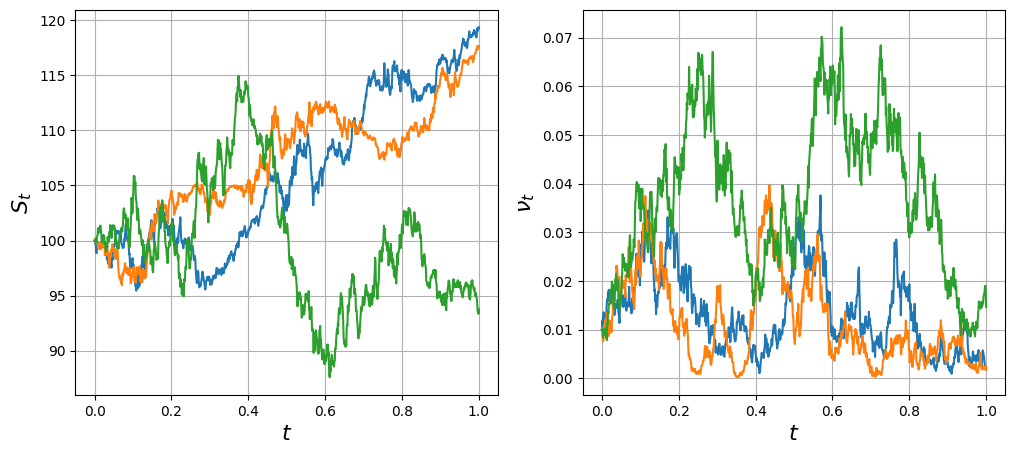
\includegraphics[scale=0.53]{fig/img/HestonModel/heston_simulationsflottere.png}
    \caption{Simulated Paths with Parameters in Table \ref{heston_tabel}.}
    \label{fig:heston_simsl}
\end{figure}

%The Heston model will serve as a comparative model for our rough volatility model.
If we let $F(t,S_{t},\nu_{t})$ denote the price function of a European call option with maturity time $T>0$ and strike price $K>0$ in the Heston model, then we can apply Itô's lemma and standard arbitrage arguments as in Section \ref{sec:BSM} to obtain Garman's partial differential equation
\begin{align*}
    &\frac{\partial F}{\partial t} + \frac{S_{t}^{2}\nu_{t}}{2}\frac{\partial^{2}F}{\partial S_{t}^{2}} + (r-q)S_{t}\frac{\partial F}{\partial S_{t}} - (r-q)F\\
    &+ \left(\kappa(\theta - \nu_{t})-\lambda \nu_{t}\right)\frac{\partial F}{\partial \nu_{t}} + \frac{\xi^{2}\nu_{t}}{2}\frac{\partial^{2}F}{\partial \nu_{t}^{2}} + \rho\xi S_{t}\nu_{t}\frac{\partial^{2}F}{\partial S_{t}\partial \nu_{t}}=0,
\end{align*}
where $r$ is the risk-free rate, $q$ is the dividend yield, and $\lambda$ is the market price of risk. As in the Black-Scholes model, we will assume that stocks don't pay dividens and therefore $q=0$. By analogy with the Black-Scholes formula \eqref{BSFormula}, we guess a solution of the form
\begin{equation}
    F(t,S_{t},\nu_{t})=S_{t}P_{1} - e^{-r(T-t)}KP_{2},
\end{equation}
where $P_{1}$ and $P_{2}$ are the conditional risk neutral probabilities of the option expiring in the money. These probabilities are not immediately available in closed-form.
%where $P_{1}$ is the delta of the option, and $P_{2}$ is the conditional risk neutral probability of the option expiring in the money, i.e. $P_{2}=\mathbb{Q}(S_{T}>K)$ for some martingale measure $\mathbb{Q}\sim \mathbb{P}$.
However, if we let $\psi_{1},\psi_{2}$ denote the characterstic functions (Fourier transforms) of $P_{1}$ and $P_{2}$, we then have that $P_{1}$ and $P_{2}$ can be computed via the inverse Fourier transform
\begin{equation}
    P_{j}=\frac{1}{2}+\frac{1}{\pi}\int_{0}^{\infty}\textrm{Re}\left[\frac{\exp\left\{-i\phi \ln K\right\}\psi_{j}}{i\phi}\right]d\phi, \quad j\in \{1,2\},
\end{equation}
where $i$ is the imaginary unit. Heston assumes the characteristic functions have the functional form
\begin{equation}
    \psi_{j}(\tau; \phi)=\exp\left\{C_{j}(\tau;\phi)+D_{j}(\tau;\phi)\nu_{0}+i\phi S_{0}\right\},\quad \tau=T-t, \hspace{6 pt}j\in\{1,2\}.
\end{equation}
If we substitute $\psi_{1}$ and $\psi_{2}$ into Garman's partial differential equation, we get the following ordinary differential equations for the unknown functions $C_{j}(\tau;\phi)$ and $D_{j}(\tau;\phi)$
\begin{align}
    &\frac{dC_{j}(\tau;\phi)}{d\tau}-\kappa\theta D_{j}(\tau;\phi) - r\phi i=0,\label{ode1}\\
    &\frac{dD_{j}(\tau;\phi)}{d\tau}-\frac{\xi^{2}D_{j}^{2}(\tau;\phi)}{2} + (b_{j}-\rho\xi\phi i)D_{j}(\tau;\phi) - u_{j}\phi i + \frac{\phi^2}{2}=0,\label{ode2}
\end{align}
where $j\in\{1,2\}$, and the initial conditions are $C_{j}(0;\phi)=D_{j}(0;\phi)=0$. The solution of the system \eqref{ode1} - \eqref{ode2} is given by
\begin{align}
    C(\tau;\phi)&=r\phi i\tau+\frac{\kappa\theta}{\xi^{2}}\left((b_{j}-\rho\xi \phi i+d)\tau -2\ln\left(\frac{1-ge^{d\tau}}{1-g}\right)\right),\\
    D(\tau;\phi)&=\frac{b_{j}-\rho\xi\phi i+d}{\xi^{2}}\left(\frac{1-e^{d\tau}}{1-ge^{d\tau}}\right),
\end{align}
where 
\begin{equation*}
    g=\frac{b_{j}-\rho\xi\phi i+d}{b_{j}-\rho\xi\phi i-d}, \quad d=\sqrt{(\rho\xi\phi i-b_{j})^{2}-\xi^{2}(2u_{j}\phi i-\phi^{2})},
\end{equation*}
with $u_{1}=1/2$, $u_{2}=-1/2$, $b_{1}=\kappa + \lambda-\rho\xi$, and $b_{2}=\kappa + \lambda$. 

As argued in \cite[p.~16]{volsurface}, we assume that the Heston process calibrated to option prices, generates the risk-neutral measure such that market price of risk $\lambda$ henceforth will be set to zero. 

\subsection{Heston Model Calibration}
Model calibration is the problem of determining the model parameters to match the market prices of a given set of options. However, in practice it is not possible nor meaningful to match the market prices exactly. Therefore, model calibration is formulated as an optimization problem, where we attempt to find the model parameters that minimize the pricing error by our model on a given set of options. One possible metric for the pricing error is the squared distance, which leads to the non-linear least squares problem
\begin{equation}\label{eq:calibration}
    \hat{\Theta}=\argmin_{\Theta}G(\Theta),\quad G(\Theta)= \sum_{i=1}^{N}w_{i}\left(F^{\Theta}_{i}(t,S_{t},T_{i},K_{i}) - F_{i}^{MP}(T_{i},K_{i})\right)^{2},
\end{equation}
where $N$ is the number of options used, $w_{i}$ are weights, $F^{MP}_{i}(T_{i},K_{i})$ is the market price of option $i$ with maturity time $T_{i}>0$ and strike price $K_{i}>0$, and $F^{\Theta}_{i}(t,S_{t},T_{i},K_{i})$ is the model price of the same option computed with the model parameters $\Theta$. For the Heston model, the parameter space is $\Theta=(\nu_{0},\kappa,\theta,\xi,\rho)\subset \R^{5}$. We simply set $w_{i}=1$ for $i=1,\dots,N$ and impose the constraints on the calibrated parameters $\hat{\Theta}=(\hat{\nu}_{0},\hat{\kappa},\hat{\theta},\hat{\xi},\hat{\rho})$ that $\hat{\nu}_{0}\in [0.001, 0.25]$, $\hat{\kappa}\in [0.001, 5]$, $\hat{\theta}\in [0.001, 0.1]$, $\hat{\xi}\in [0.01, 1]$, and $\hat{\rho}\in [-0.99, 0.99]$ with initial guesses $\hat{\Theta}_{0}=(0.1, 3, 0.05, 0.3, -0.8)$. Additionally, we set to the tolerance for termination to $0.001$. We use an extension of the limited-memory BFGS algorithm, which can handle the box constraints just imposed on the parameter space, to solve the optimization problem \eqref{eq:calibration}.
%Applying Itô's lemma and standard arbitrage arguments as in Section \ref{sec:BSM}, we obtain the 
\section{Implied Volatility}
This section is based on \cite{impvol}.

If we consider the Black \& Scholes price function $F$ given by \eqref{BSFormula}, then we could reparameterize it, and instead consider $F$ as a function of $(\tau, y, \sigma)$, where $\tau=T-t$ is time to maturity, $y=S_{t}/K$ is the so-called moneyness, and $\sigma$ is the volatility term. These quantities are all observable except for $\sigma$. However, the mapping $\sigma\mapsto F(t,S_{t},\sigma)$ is continuous and strictly increasing on $(0,\infty)$, and consequently also invertible on $(0,\infty)$. Hence, there is a one-to-one correspondence between the price of an option and the volatility of the underlying stock. This leads us to the concept of implied volatility.
\begin{defn}[\textit{Implied Volatility}]
    Let $F$ be the Black \& Scholes price function for a European call option. If $F^{MP}(t, K)$ denotes the market price of a European call option with time to maturity $\tau=T-t$ and moneyness $y=S_{t}/K$, then the implied volatility of the option is defined as the unique number $\sigma_{BS}(\tau, y)>0$, which satisfies
    \begin{equation}\label{eq:impvol}
        F^{MP}(t,K)=F\left(T-\tau, \hspace{1 pt}yK,\hspace{1 pt}\sigma_{BS}(\tau,y)\right).
    \end{equation}
\end{defn}
In practice, we compute the implied volatility numerically using a root-finding algorithm such as the Newton-Raphson method to find the number $\sigma_{BS}(\tau,y)>0$ that satisfies \eqref{eq:impvol}. 

Intuitively, implied volatility is the market's forecast of the future volatility of the underlying asset, and can be thought of as a proxy of market risk. It is important to note that although implied volatility helps quantify market sentiment, it doesn't actually predict the direction nor magnitude of the price fluctuations of the underlying asset. If an investor wants to gain an overview of how the implied volatility changes with respect to the strike price and the time to maturity, they can look at the implied volatility surface. Such a surface is seen in Figure \ref{fig:impVolsurf}, which shows the implied volatility of options written on the SPDR S\&P 500 ETF (SPY) with expiration dates ranging from 6/12-2023 to 21/3-2025.
\begin{figure}[H]
    \centering
    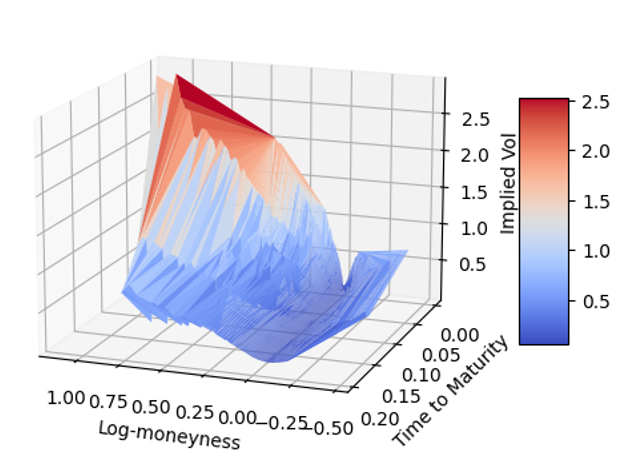
\includegraphics[scale=0.75]{fig/img/ImpliedVol/vol_surface_lidtflottereigen.PNG}
    \caption{Implied Volatility Surface, SPY ETF.}
    \label{fig:impVolsurf}
\end{figure}
In Figure \ref{fig:impVolsurf}, it is seen that for options at-the-money (ATM) with $\ln(S_{t}/K)=0$, there is a certain symmetry around ATM, which gets more pronounced closer to maturity. Intuitively, this means that ATM options have lower implied volatility than options out-the-money (OTM) or in-the-money (ITM). In Figure \ref{fig:impVolsurf}, the ITM have higher implied volatilities than those OTM, which gives rise to the so-called volatility skew observed. If the surface was symmetric around ATM, we would observe a so-called volatility smile. Examples of both a volatility smile and volatility skew are seen in Figure \ref{fig:smileskew} below.
\begin{figure}[H]
    \centering
    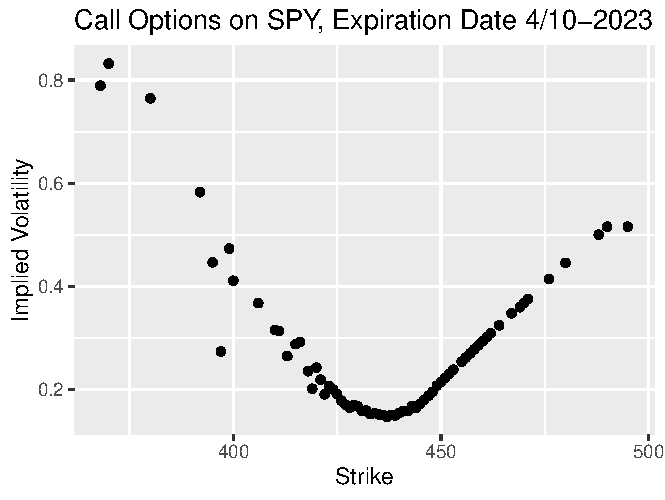
\includegraphics[scale=0.6]{fig/img/ImpliedVol/VolSmile20231003.pdf}
    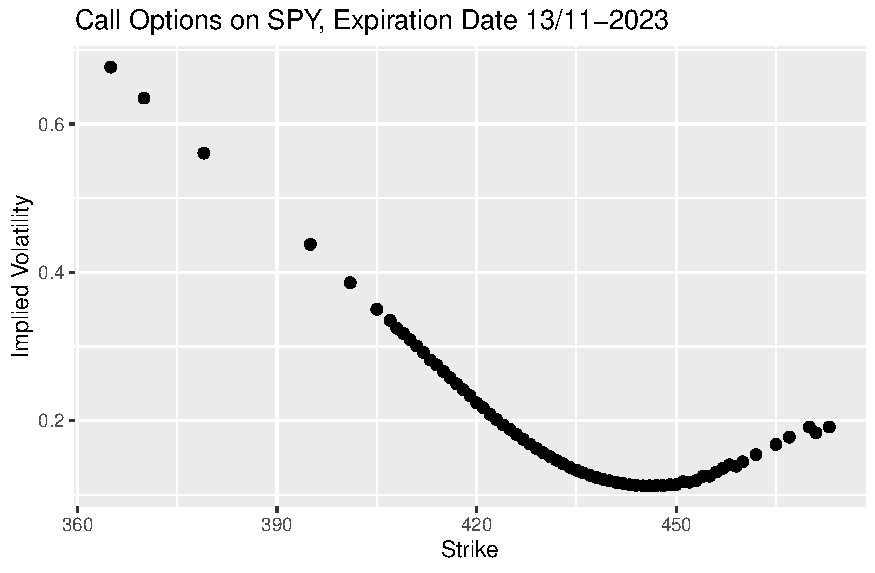
\includegraphics[scale=0.52]{fig/img/ImpliedVol/VolSkewNov13.pdf}
    \caption{Volatility Smile (left) and Volatility Skew (right).}
    \label{fig:smileskew}
\end{figure}
\section{Fractional Brownian Motion}
This section is based on \cite{fBMbook}.

In this section, we assume that every random variable $X_{t}$ is defined on some appropriate probability space $(\Omega, \mathcal{F},\mathbb{P})$. Furthermore, we assume that the index set $I$ is either equal to $\R$, $[0,\infty)$ or $[0,T]$ for some $T>0$. 
\begin{defn}[\textit{Gaussian Process}]
    A stochastic process $X=(X_{t})_{t\in I}$ is said to be Gaussian if for all $d\geq 1$ and all $t_{1},\dots,t_{d}\in I$, $(X_{t_{1}},\dots,X_{t_{d}})$ is a Gaussian random vector. The mean function $m: I\to \R$ of $X$ is given by $m(t)=\mathbb{E}[X_{t}]$, and the covariance function $\gamma: I^{2}\to\R$ of $X$ is given by $\gamma(s,t)=\textrm{Cov}(X_{s},X_{t})$. If $m\equiv 0$, $X $ is said to be centered.
\end{defn}

\begin{defn}[\textit{Positive Semidefinite Function}]
    A symmetric function $\gamma: I^{2}\to \R$ is said to be positive semidefinite if
    \begin{equation}\label{posdef}
        \sum_{i=1}^{d}\sum_{j=1}^{d}a_{i}a_{j}\gamma(t_{i},t_{j})\geq 0
    \end{equation}
    for all $d\geq 1$, $t_{1},\dots,t_{d}\in I$, and $a_{1},\dots,a_{d}\in\R$.
\end{defn}
In fact, the condition \eqref{posdef} is equivalent to the matrix $\Gamma=\big\{\gamma (t_{i},t_{j})\big\}_{i,j=1}^{d}$ being a positive semidefinite matrix for all $d\geq 1$ and $t_{1},\dots,t_{d}\in I$.

\begin{thm}[\textit{Kolmogorov}]\label{kolmogorov}
    Let $\gamma: I^{2}\to\R$ be a symmetric function. Then there exists a centered Gaussian process $X=(X_{t})_{t\in I}$ having $\gamma$ for covariance function, if and only if $\gamma$ is positive semidefinite.
\end{thm}
\begin{lem}[\textit{Kolmogorov-Centsov}]
    Let $I=[0,T]\subset [0,\infty)$ be a compact interval for $T>0$, and let $X=(X_{t})_{t\in I}$ be a centered Gaussian process. Suppose there exists $C,\eta>0$ such that for all $s,t\in I$
    \begin{equation}
        \mathbb{E}\left[(X_{t}-X_{s})^{2}\right]\leq C|t-s|^{\eta}.
    \end{equation}
    Then, for all $\alpha\in (0,\eta/2)$, there exists a continuous modification $Y$ of $X$ with $\alpha$-Hölder continuous path. In particular, $X$ admits a continuous modification.
\end{lem}
The $\alpha$-Hölder continuity of the paths of $Y$ means there exists $C_{\alpha}\geq 0$ such that
\begin{equation}
    |Y_{t}(\omega)-Y_{s}(\omega)|\leq C_{\alpha}|t-s|^{\alpha},\quad \forall s,t\in I,\hspace{2 pt}\forall\omega\in\Omega\setminus N,
\end{equation}
where $N$ is a $\mathbb{P}$-zero set.
\begin{thm}
  Let $H>0$ be a real parameter. Then there exists a continuous centered Gaussian process $B^{H}=(B_{t}^{H})_{t\geq 0}$ with covariance function
  \begin{equation}
      \gamma_{H}(t,s)=\frac{1}{2}(t^{2H}+s^{2H}-|t-s|^{2H}), \quad s,t\geq 0,
  \end{equation}
  if and only if $H\leq 1$. In this case, the paths of $B^{H}$ are $\alpha$-Hölder continuous on each compact set $I\subset [0,\infty)$ for any $\alpha\in (0,H)$.
\end{thm}
\begin{proof}
    According to the Kolmogorov Theorem \ref{kolmogorov}, to show the existence of $B^{H}$, we have to show that $\gamma_{H}$ is positive semidefinite if and only $H\leq 1$.
    Assume first that $H>1$, and take $t_{1}=1$, $t_{2}=2$, $a_{1}=-2$, and $a_{2}=1$. Then consider
    \begin{align}
        a_{1}^{2}\gamma_{H}(t_{1},t_{1})+2a_{1}a_{2}\gamma_{H}(t_{1},t_{2})+a_{2}^{2}\gamma_{H}(t_{2},t_{2})=4-2^{2H}<0.
    \end{align}
    Thus, $\gamma_{H}$ is not positive semidefinite when $H>1$. If $H=1$, then $\gamma_{1}(s,t)=st$ is indeed positive semidefinite such that for all $d\geq 1$, $t_{1},\dots,t_{d}\geq 0$, and $a_{1},\dots,a_{d}\in \R$
    \begin{equation}
        \sum_{i=1}^{d}\sum_{j=1}^{d}a_{i}a_{j}\gamma_{1}(t_{i},t_{j})= \left(\sum_{i=1}^{d}t_{i}a_{i}\right)^{2}\geq 0.
    \end{equation}
    Suppose $H\in (0,1)$
\end{proof}
\begin{defn}[\textit{Fractional Brownian Motion}]
    Let $H\in (0,1]$. A fractional Brownian motion (fBM) of Hurst index $H$ is a continuous centerede Gaussian process $B^{H}=(B_{t}^{H})_{t\geq 0}$ with covariance function
    \begin{equation}
        \gamma_{H}(t,s)=\mathbb{E}[B_{t}^{H}B_{s}^{H}]=\frac{1}{2}\left(t^{2H}+s^{2H}-|t-s|^{2H}\right).
    \end{equation}
\end{defn}
Proposition \ref{prop211} and \ref{prop212} exhibit some properties of the fractional Brownian motion.
\begin{prop}\label{prop211}
    Let $B^{H}$ be a fractional Brownian motion of Hurst index $H\in (0,1]$.
    \begin{enumerate}
        \item If $H=1/2$, then $B^{H}$ is just a standard Brownian motion.
        \item If $H=1$, then $B^{H}_{t}=tB_{1}^{H}$ almost surely for all $t\geq 0$.
    \end{enumerate}
\end{prop}
\begin{proof}
    For $H=1/2$, we immediately see that
    \begin{align}
        \mathbb{E}[B_{t}^{1/2}B_{s}^{1/2}]&=\frac{1}{2}\left(t+s-|t-s|\right)\\
        &= \frac{1}{2}\left(t+s-2 \min\{s,t\}-s-t\right)\\
        &= s\land t,
    \end{align}
    so $B^{1/2}$ is a standard Brownian motion.

    Let $H=1$. Then for all $t\geq 0$, we have
    \begin{align}
        \mathbb{E}\left[(B^{1}_{t}-tB_{1}^{1})^{2}\right]&= \mathbb{E}\left[(B_{t}^{1})^{2}\right]-2t\mathbb{E}\left[B_{t}^{1}B_{1}^{1}\right]+t^{2}\mathbb{E}\left[(B_{1}^{1})^{2}\right]\\
        &= t^{2}-t\left(t^{2}+1-(1-t)^{2}\right)+t^{2}\\
        &= 0,
    \end{align}
    so $B_{t}^{1}=tB_{1}^{1}$ almost surely.
\end{proof}
In particular, Proposition \ref{prop211} shows that it suffices to only consider fractional Brownian motions with Hurst index $H\in (0,1)$.
 \begin{prop}\label{prop212}
     Let $B^{H}$ be a fractional Brownian motion of Hurst index $H\in (0,1)$. Then we have
     \begin{enumerate}
         \item (Self-similarity) For all $a>0$, $\left(a^{-H}B^{H}_{at}\right)_{t\geq 0}\mylaw(B_{t}^{H})_{t\geq 0}$.
         \item (Stationarity of Increments) For all $h>0$, $\left(B_{t+h}^{H}-B_{h}^{H}\right)_{t\geq 0}\mylaw (B_{t}^{H})_{t\geq 0}$.
         \item (Time Inversion) $\left(t^{2H}B^{H}_{1/t}\right)_{t>0}\mylaw (B_{t}^{H})_{t>0}$.
     \end{enumerate}
     Conversely, any continuous Gaussian process $B^{H}=(B_{t}^{H})_{t\geq 0}$ with $B_{0}^{H}=0$, $\textrm{Var}[B_{1}^{H}]=1$, and such that 1. and 2. above hold, is a fractional Brownian motion of Hurst index $H$.
 \end{prop}
 \begin{proof}
 To prove self-similarity, we see that
     \begin{align}
         \mathbb{E}\left[a^{-H}B_{at}^{H}a^{-H}B_{as}^{H}\right]&=a^{-2H}\mathbb{E}[B_{at}^{H}B_{as}^{H}]\\
         &=\frac{a^{-2H}}{2}\left((at)^{2H}+(as)^{2H}-|at-as|^{2H}\right)\\
         &= \frac{1}{2}(t^{2H}+s^{2H}-|t-s|^{2H}).
     \end{align}
     The proof of 2. and 3. are completely analogous, and are therefore omitted. Conversely, let $B^{H}=(B_{t}^{H})_{t\geq 0}$ be a continuous Gaussian process with $B^{H}_{0}=0$ and $\textrm{Var}[B_{1}^{H}]=1$, which additionally satisfies 1. and 2. Using 2. with $t=h>0$, we get $\mathbb{E}[B_{2t}^{H}]=2\mathbb{E}[B_{t}^{H}]$, and using 1. we infer that $\mathbb{E}[B_{2t}^{H}]=2^{H}\mathbb{E}[B_{t}^{H}]$. Combining these two equalities gives $\mathbb{E}[B_{t}^{H}]=0$ for all $t>0$, and thus $B^{H}$ is centered. Let $s,t\geq 0$. Then we infer that
     \begin{align}
         \E[B_{s}^{H}B_{t}^{H}]&=\frac{1}{2}\left(\E\left[(B_{t}^{H})^{2}\right]+\E\left[(B_{s}^{H})^{2}\right]-\E\left[(B_{t}^{H}-B_{s}^{H})^{2}\right]\right)\\
         &= \frac{1}{2}\left(\E\left[(B_{t}^{H})^{2}\right]+\E\left[(B_{s}^{H})^{2}\right]-\E[(B_{|t-s|}^{H})^{2}]\right)\\
         &= \frac{1}{2}\E[(B_{1}^{H})^{2}]\left(t^{2H}+s^{2H}-|t-s|^{2H}\right)\\
         &= \frac{1}{2}\left(t^{2H}+s^{2H}-|t-s|^{2H}\right),
     \end{align}
     which concludes the proof.
 \end{proof}
\begin{defn}[\textit{Fractional Gaussian Noise}]
    Let $B^{H}= (B_{t}^{H})_{t\geq 0}$ be a fractional Gaussian process of Hurst index $H\in (0,1)$. Then the increments defined as
    \begin{equation}
        \Delta B_{t}^{H}\coloneqq B_{t+h}^{H}-B_{t}^{H}, \quad h>0,
    \end{equation}
    are called fractional Gaussian noise.
\end{defn}
We have the following proposition.
\begin{prop}\label{corr}
    Let $B^{H}=(B_{t}^{H})_{t\geq 0}$ be a fractional Brownian motion of Hurst index $H\in (0,1)$. Then disjoint increments of $B^H$ are negatively correlated for $H\in (0,1/2)$, positively correlated for $H\in (1/2,1)$, and uncorrelated for $H=1/2$.
\end{prop}
\begin{proof}
Let $\Delta B_{t}^{H}=B_{t+h}^{H}-B_{t}^{H}$ and $\Delta B_{s}^{H}=B_{s+h}^{H}-B_{s}^{H}$ be increments of a fractional Brownian motion $B^{H}$ such that $s+h< t$ and $t-s=nh$, $n\in \N$ so as to ensure $[s,s+h]\cap [t,t+h]=\emptyset$. Then the covariance of the increments is given as
\begin{align*}
    \E\left[\Delta B_{t}^{H}\Delta B_{s}^{H}\right]&=\E[B_{t+h}^{H}B_{s+h}^{H}]-\E[B_{t+h}^{H}B_{s}^{H}]-\E[B_{t}^{H}B_{s+h}^{H}]+\E[B_{t}^{H}B_{s}^{H}]\\
    &= \frac{1}{2}\left((t+h)^{2H}+(s+h)^{2H}-|nh|^{2H}\right)-\frac{1}{2}\left((t+h)^{2H}+s^{2H}-|h(n+1)|^{2H}\right)\\
    & -\frac{1}{2}\left(t^{2H}+(s+h)^{2H}-|h(n-1)|^{2H}\right)+ \frac{1}{2}\left(t^{2H}+s^{2H}-|nh|^{2H}\right)\\
    &=  \frac{1}{2}h^{2H}\left((n+1)^{2H}+(n-1)^{2H}-2n^{2H}\right).
\end{align*}
Thus, for a fixed $h$, the covariance of the increments only depends on $n\in \N$. Define the function $f:[1,\infty)\to \R$ by
\begin{equation}
f(x)\coloneqq (x+1)^{2H}+(x-1)^{2H}-2x^{2H}.
\end{equation}
Then, it is easy to see that $f(x)>0$, $\forall x\in [1,\infty)$ if $H>1/2$, and $f(x)<0$, $\forall x\in [1,\infty)$ if $H<1/2$. In the case of $H=1/2$, the increments are independent, and by virtue of the Brownian motion being a Gaussian process, they are consequently also uncorrelated.
    %Suppose that $0\leq s_{1}<t_{1}<s_{2}<t_{2}$ such that $[s_{1},t_
    %{1}]\cap [s_{2},t_{2}]=\emptyset$. Then the covariance of the increments is given as
    %\begin{align*}
        %\E\left[(B_{t_{1}}^{H}-B_{s_{1}}^{H})(B_{t_{2}}^{H}-B_{s_{2}}^{H})\right] &= \E[B_{t_{1}}^{H}B_{t_{2}}^{H}]-\E[B_{t_{2}}^{H}B_{s_{1}}^{H}]-\E[B_{t_{1}}^{H}B_{s_{2}}^{H}] + \E[B_{s_{1}}^{H}B_{s_{2}}^{H}]\\
        %&= \frac{1}{2}\left(|t_{2}-s_{1}|^{2H}-|t_{2}-t_{1}|^{2H}-\left(|s_{2}-s_{1}|^{2H}-|s_{2}-t_{2}|^{2H}\right)\right).
    %\end{align*}
    %Now, define the function $f(x)=|x|^{2H}$ and put $a_{1}\coloneqq t_{2}-s_{1}$, $a_{2}\coloneqq t_{2}-t_{1}$, $b_{1}\coloneqq s_{2}-s_{1}$, and $b_{2}\coloneqq s_{2}-t_{2}$. Note that $b_{2}<a_{2}<b_{1}<a_{1}$. This allows the covariance of the increments to be expressed as 
    %\begin{equation}
        %\E\left[(B_{t_{1}}^{H}-B_{s_{1}}^{H})(B_{t_{2}}^{H}-B_{s_{2}}^{H})\right]=\frac{1}{2}\left(f(a_{1})-f(a_{2})-\left(f(b_{1})-f(b_{2})\right)\right).
    %\end{equation}
\end{proof}
It is well-known that a discrete stationary stochatic process $(X_{n})_{n\in \N}$ is said to exhibit long memory if its autocovariance function $\rho(n)\coloneqq \textrm{Cov}(X_{k},X_{k+n})$ satisfies $\rho(n)\sim cn^{-\alpha}$, i.e.
\begin{equation}
    \lim_{n\to \infty}\frac{\rho(n)}{cn^{-\alpha}}=1,
\end{equation}
for some constant $c$ and $\alpha \in (0,1)$. In this case, we have that $\sum_{n=1}^{\infty}\rho(n)=\infty$. Consequently, we obtain that the increments $X_{k}\coloneqq B^{H}_{k}-B^{H}_{k-1}$ and $X_{k+n}\coloneqq B^{H}_{k+n}-B^{H}_{k+n-1}$ of a fBM $B^H$ exhibit long memory for $H>1/2$, since 
\begin{equation}\label{asymp}
    \rho_{H}(n)\coloneqq \frac{1}{2}\left((n+1)^{2H}+(n-1)^{2H}-2n^{2H}\right) \sim H(2H-1)n^{2H-2},
\end{equation}
as $n\to \infty$. Thus, we obtain that $\sum_{n=1}^{\infty}\rho_{H}(n)=\infty$ for $H>1/2$, and $\sum_{n=1}^{\infty}|\rho_{H}(n)|<\infty$ for $H<1/2$.
\section{Semimartingale Property}
In this section, we will study the asymptotic properties of the $p$-variations of a fBM. Additionally, we will show that a fBM is not a semimartingale except for when $H=1/2$. Firstly, we introduce the class of Hermite polynomials and a useful lemma.
\begin{defn}[\textit{Hermite Polynomials}]
    The Hermite polynomials are defined as the family $(H_{k})_{k\in \N}\subset \R[x]$ of polynomials satisfying
    \begin{equation}
        H_{k}(x)=(\delta^{k}1)(x), \quad k\in\N,
    \end{equation}
    where $1$ is the function constantly equal to $1$, and $(\delta\varphi)(x)\coloneqq x\varphi(x)-\varphi'(x)$ for $\varphi\in C^{1}$.
\end{defn}
\begin{lem}\label{l2lemma}
    Let $(h_{k})_{k\in \N}$ be the family of Hermite polynomials. Then $(\frac{1}{\sqrt{k!}}H_{k})_{k\in\N}$ is an orthonormal basis of $L^{2}\left(\R,\mathcal{B}(\R),\nu\right)$, where $\nu$ is the standard Gaussian measure
    \begin{equation}
        \nu(A)\coloneqq \frac{1}{\sqrt{2\pi}}\int_{A}e^{-x^{2}/2}dx,\quad A\in\mathcal{B}(\R).
    \end{equation}
\end{lem}
We present the following theorem, which may be viewed as a law of large numbers for fractional Brownian motions.
\begin{thm}\label{llnthm}
    Let $G\sim\mathcal{N}(0,1)$ and let $f:\R\to\R$ be a measurable function such that $\E[f^{2}(G)]<\infty$. Let $B^H$ be a fractional Brownian motion of Hurst index $H\in (0,1)$. Then, as $n\to\infty$
    \begin{equation}\label{lln}
        \frac{1}{n}\sum_{i=1}^{n}f(B^{H}_{i}-B^{H}_{i-1})\overset{L^{2}}{\to} \E[f(G)]
    \end{equation}
\end{thm}
Note that using the self-similariy property, we can rewrite \eqref{lln} as
\begin{equation}
     \frac{1}{n}\sum_{i=1}^{n}f\left(n^{H}(B^{H}_{i/n}-B^{H}_{(i-1)/n})\right)\overset{L^{2}}{\to} \E[f(G)] \hspace{6 pt}\mathrm{as}\hspace{5 pt}n\to\infty.
\end{equation}
\begin{proof}
    If $H=1/2$, then the result follows from the classical law of large numbers, since the increments then $B^{1/2}_{i}-B^{1/2}_{i-1}\overset{\textrm{i.i.d}}{\sim} \mathcal{N}(0,1)$. Assume now that $H\neq 1/2$. Since $\E[f^{2}(G)]<\infty$, we have that $f\in L^{2}\left(\R,\mathcal{B}(\R),\nu\right)$, and as a consequence of Lemma \ref{l2lemma}
    \begin{equation}\label{infsum}
        f(x)=\sum_{k=0}^{\infty}\frac{c_{k}}{\sqrt{k!}}H_{k}(x), \quad x\in \R,
    \end{equation}
    where $H_{0}(x)\equiv 1$. By the orthogonality of the Hermite polynomials, we have $\sum_{k=0}^{\infty}c_{k}^{2}=\E[f^{2}(G)]<\infty$. Choosing $x=G$ and taking the expectation in $\eqref{infsum}$, we obtain that $c_{0}=\E[f(G)]$. Hence
    \begin{align}
        \frac{1}{n}\sum_{i=1}^{n}f(B_{i}^{H}-B_{i-1}^{H}) - \E[f(G)]&=\frac{1}{n}\sum_{i=1}^{n}\left(f(B_{i}^{H}-B_{i-1}^{H}) - \E[f(G)]\right)\\
        &= \frac{1}{n}\sum_{k=0}^{\infty}\frac{c_{k}}{\sqrt{k!}}\sum_{i=1}^{n}H_{k}(B_{i}^{H}-B_{i-1}^{H}).
    \end{align}
In the following, we will use the fact that if $(U,V)$ is a Gaussian vector with $U,V\sim\mathcal{N}(0,1)$, then for all $k,l\in\N$
\begin{equation}\label{fintresultat}
    \E[H_{k}(U)H_{l}(V)]=\begin{cases}
        k!\E[UV]^{k} & \mathrm{if}\hspace{2.5 pt} k=l,\\
        0, & \mathrm{otherwise}.
    \end{cases}
\end{equation}
Using \eqref{fintresultat}, we deduce
\begin{align}
    &\E\left[\left(\frac{1}{n}\sum_{i=1}^{n}f(B_{i}^{H}-B_{i-1}^{H}) - \E[f(G)]\right)^{2}\right]\\
    &= \frac{1}{n^2}\sum_{k=1}^{\infty}\frac{c_{k}^{2}}{k!}\sum_{i'=1}^{n}\sum_{i =1}^{n}\E[H_{k}(B^{H}_{i}-B_{i-1}^{H})H_{k}(B^{H}_{i'}-B^{H}_{i'-1})]\\
    &= \frac{1}{n^2}\sum_{k=1}^{\infty}c_{k}^{2}\sum_{i'=1}^{n}\sum_{i =1}^{n}\E[(B^{H}_{i}-B_{i-1}^{H})(B^{H}_{i'}-B^{H}_{i'-1})]^{k}\\
    &= \frac{1}{n^2}\sum_{k=1}^{\infty}c_{l}^{2}\sum_{i'=1}^{n}\sum_{i =1}^{n}\rho_{H}(i-i')^{k},
\end{align}
where $\rho_{H}$ is the autocovariance function of fractional Gaussian noise
\begin{equation}
    \rho_{H}(x)=\rho_{H}(|x|)=\frac{1}{2}\left(|x+1|^{2H}+|x-1|^{2H}-2|x|^{2H}\right), \quad x\in \Z. 
\end{equation}
Utilizing the fact that $\rho_{H}(x)=\E[B_{1}^{H}(B_{|x|+1}^{H}-B_{|x|}^{H})]$, and that the covariance is an inner product, we get by Cauchy-Schwarz
\begin{align}
     |\rho_{H}(x)|\leq \sqrt{\E[(B_{1}^{H})^{2}]}\sqrt{\E[(B_{|x|+1}^{H}-B_{|x|}^{H})^{2}]}=1.
\end{align}
We are now ready to study the $L^2$-convergence of $n^{-1}\sum_{i=1}^{n}f(B_{i}^{H}-B_{i-1}^{H})-\E[f(G)]$
\begin{align}
    \E\left[\left(\frac{1}{n}\sum_{i=1}^{n}f(B_{i}^{H}-B_{i-1}^{H})-\E[f(G)]\right)^{2}\right] &\leq \frac{1}{n^{2}}\sum_{k=1}^{\infty}c_{k}^{2}\sum_{i'=1}^{n}\sum_{i =1}^{n}|\rho_{H}(i-i')|\\
    &= \mathrm{Var}[f(G)]\frac{1}{n^2}\sum_{i'=1}^{n}\sum_{i =1}^{n}|\rho_{H}(i-i')|\\
    &= \mathrm{Var}[f(G)]\frac{1}{n^2}\sum_{i'=1}^{n}\sum_{i=1-i'}^{n-i'}|\rho_{H}(i)|\\
    &\leq 2\mathrm{Var}[f(G)]\frac{1}{n}\sum_{i=0}^{n-1}|\rho_{H}(i)|.
\end{align}
We already know from \eqref{asymp} that $\rho_{H}(i)\sim H(2H-1)i^{2H-2}$ as $i\to \infty$. We know that if $H<1/2$, then $\sum_{i=1}^{\infty}|\rho_{H}(i)|<\infty$, and the result \eqref{lln} holds. If $H>1/2$, then $\sum_{i=1}^{n-1}|\rho_{H}(i)|\sim H(2H-1)\sum_{i=1}^{n-1}i^{2H-2}\sim Hn^{2H-1}$ as $n\to \infty$, and the result \eqref{lln} holds as well because $H<1$.
\end{proof}
As a consequence, we have the following corollary.
\begin{cor}\label{pvariations}
    Let $B^H$ be a fractional Brownian motion of Hurst index $H\in (0,1)$, and let $p\in [1,\infty)$. Then, in $L^{2}(\Omega,\mathcal{F},\mathbb{P})$ and as $n\to\infty$, we have
    \begin{equation}
        \sum_{i=1}^{n}\left|B_{i/n}^{H}-B_{(i-1)/n}^{H}\right|^{p}\to \begin{cases}
            0, & \mathrm{if} \hspace{3 pt}p>\frac{1}{H},\\
            \E[|G|^{p}], & \mathrm{if}\hspace{3 pt}p=\frac{1}{H},\hspace{3 pt} \mathrm{with}\hspace{3 pt} G\sim \mathcal{N}(0,1),\\
            \infty, & \mathrm{if}\hspace{3 pt}p<\frac{1}{H}.
        \end{cases}
    \end{equation}
\end{cor}
\begin{proof}
    If we apply Theorem \ref{llnthm} with $f(x)=|x|^p$, we get
    \begin{align}
         \sum_{i=1}^{n}\left|B_{i/n}^{H}-B_{(i-1)/n}^{H}\right|^{p}&= \sum_{i=1}^{n}\left|n^{-H}(B_{i}^{H}-B_{i-1}^{H})\right|^{p}\\
         &= \frac{1}{n^{Hp}}\sum_{i=1}^{n}\left|B_{i}^{H}-B_{i-1}^{H}\right|^{p}\\
         &= \frac{1}{n^{H(p-1/H)}}\left(\frac{1}{n}\sum_{i=1}^{n}\left|B_{i}^{H}-B_{i-1}^{H}\right|^{p}\right)\\
         &= \frac{1}{n^{H(p-1/H)}}\E[f(G)].
    \end{align}
If $p=1/H$, then the above is simply equal to \eqref{lln}. If $p<1/H$, then $n^{-H(p-1/H)}\to \infty$ as $n\to \infty$, and conversely $n^{-H(p-1/H)}\to 0$ as $n\to \infty$ if $p>1/H$.
\end{proof}
We are now ready to prove that a fBM is not a semimartingale, except when $H=1/2$. Consequently, integration with respect to a fBM becomes a non-trivial problem, when $H\neq 1/2$.
\begin{thm}
    Let $B^H$ be a fractional Brownian motion of Hurst index $H\in (0,\frac{1}{2})\cup (\frac{1}{2},1)$. Then $B^H$ is not a semimartingale.
\end{thm}
\begin{proof}
    By selfsimilarity, it is sufficient to consider the time interval $[0,1]$ for the proof. Firstly, recall that the following two properties hold for a semimartingale $S$ on $[0,1]$
    \begin{enumerate}
        \item $\sum_{k=1}^{n}\left(S_{k/n}-S_{(k-1)/n}\right)^{2}\overset{\mathbb{P}}{\to} \langle S\rangle_{1}<\infty$ as $n\to\infty$.
        \item Moreover, if $\langle S\rangle_{1}=0$, then $S$ is of bounded variation, i.e. it holds almost surely that
        \begin{equation}
            \sup_{n\geq 1}\sum_{k=1}^{n}|S_{k/n}-S_{(k-1)/n}|<\infty. 
        \end{equation}
    \end{enumerate}
    Now, if $H<1/2$, then $\sum_{k=1}^{n}(B_{k/n}^{H}-B_{(k-1)/n}^{H})^{2}\to \infty$ by Corollary \ref{pvariations}. Hence, $B^H$ is not a semimartingale. Conversely, if $H>1/2$, then Corollary \ref{pvariations} yields $\sum_{k=1}^{n}(B_{k/n}^{H}-B_{(k-1)/n}^{H})^{2}\to 0$. Let $p\in (1,1/H)$, then Corollary \ref{pvariations} again yields $\sum_{k=1}^{n}(B_{k/n}^{H}-B_{(k-1)/n}^{H})^{p}\to \infty$. Additionally, by the uniform continuity of the paths $[0,1]\ni t\mapsto B_{t}^{H}(\omega)$, we obtain almost surely
    \begin{equation}
        \sup_{1\leq k\leq n}|B_{k/n}^{H}-B_{(k-1)/n}^{H}|^{p-1}<\varepsilon, \quad \forall \varepsilon>0.
    \end{equation}
    Combining the above, we ge the inequality
    \begin{equation}
        \sum_{k=1}^{n}\left|B_{k/n}^{H}-B_{(k-1)/n}^{H}\right|^{p}\leq \sup_{1\leq k\leq n}|B_{k/n}^{H}-B_{(k-1)/n}^{H}|^{p-1}\sum_{k=1}^{n}\left|B_{k/n}^{H}-B_{(k-1)/n}^{H}\right|
    \end{equation}
    from which we deduce that $\sum_{k=1}^{n}|B_{k/n}^{H}-B_{(k-1)/n}^{H}|\to \infty$. Consequently, $B^H$ is also not a semimartingale, when $H>1/2$.
\end{proof}
\section{Integration with Respect to Fractional Brownian Motion}
\section{Simulation of a Fractional Brownian Motion}
As was established in Proposition \ref{corr}, the increments of a fractional Brownian motion are correlated, whenever $H\neq 1/2$. Thus, the usual simulation procedure for standard Brownian motions, which consists of taking cumulative sums of i.i.d. standard normal variables, is no longer applicable. 

Suppose we wish to simulate the path of a fBM $B^{H}$ on the interval $[0,T]$ for some $T>0$. Since it is only possible to sample at a finite number of points, we will adopt the notation $Y_{t_{0}},Y_{t_{1}},\dots,Y_{t_{N}}$ for a simulated sample of $B^H$ at the points $0=t_{0}<t_{1}<\dots<t_{N}=T$. Then $(Y_{t_{0}},Y_{t_{1}},\dots,Y_{t_{N}})$ forms a centered Gaussian vector with a certain covariance matrix. Therefore, it can be simulated as a linear transform of a standard Gaussian vector, i.e. a vector of i.i.d. standard normal variables. This basic idea will be utilized in both simulation procedures presented, which are the Cholesky decomposition method and the circulant embedding method. 

Note that due to the self-similarity property, it is suffcient to simulate $(Y_{0},Y_{1},\dots, Y_{N})$ and then multiply these values by $(T/N)^H$. Furthermore, both methods presented are exact simulation techniques in the sense that if $(B_{t_{0}}^{H},B_{t_{1}}^{H},\dots, B_{t_{N}}^{H})$ is a sample from a fBM $B^H$, then 
\begin{equation}
    (Y_{t_{0}},Y_{t_{1}},\dots,Y_{t_{N}}) \overset{d}{=}(B_{t_{0}}^{H},B_{t_{1}}^{H},\dots, B_{t_{N}}^{H})
\end{equation}
as opposed to techniques that simulate with error.
%As shown in Proposition \ref{corr}, the increments of a fBM $B^{H}=(B_{t}^{H})_{t\geq 0}$ are correlated, whenever $H\neq 1/2$. This complicates the simulation of fBM's substantially, since it is no longer possible to simulate by taking cumulative sums of appropriately scaled i.i.d. standard normal variables as when simulating standard Brownian motions. In this section, two simulation methods for the fBM will be introduced, namely the Cholesky method and the circulant embedding method.

%Since it is only possible to sample at a finite number of points, we will adopt the notation $Y_{t_{0}},Y_{t_{1}},\dots,Y_{t_{N}}$ for a simulated sample of $B^{H}$ at the points $0=t_{0}<t_{1}<\dots <t_{N}=T$, where $T>0$. Furthermore, both methods presented are exact simulation techniques in the sense that if $(B_{t_{0}}^{H},B_{t_{1}}^{H},\dots, B_{t_{N}}^{H})$ is a sample from a fBM $B^H$, then
%\begin{equation}
    %(Y_{t_{0}},Y_{t_{1}},\dots,Y_{t_{N}}) \overset{d}{=}(B_{t_{0}}^{H},B_{t_{1}}^{H},\dots, B_{t_{N}}^{H})
%\end{equation}
%as opposed to simulation techniques that sample with error.
\subsection{The Cholesky Decomposition Method}
%Let $0=t_{0}<t_{1}<\dots <t_{N}=T$ be an equidistant partition of the interval $[0,T]$. 
As was established in Proposition \ref{corr}, the increments of a fBM $X_{1}=B_{1}^{H},X_{2}=B_{2}^{H}-B_{1}^{H}, \dots, X_{N}=B_{N}^{H}-B_{N-1}^{H}$ are stationary with autocovariance function
\begin{equation}
    \gamma(k)=\frac{1}{2}\left((k+1)^{2H}+|k-1|^{2H}-2k^{2H}\right), \quad k\in\N_{0}.
\end{equation}
Hence, $X=(X_{1}, X_{2},\dots,X_{N})$ forms a stationary centered Gaussian vector with covariance matrix
\begin{equation}
    \Gamma_{N}=\begin{pmatrix}
        1 & \gamma(1) & \gamma(2) & \dots & \gamma(N-2) & \gamma(N-1)\\
        \gamma(1) & 1 & \gamma(1) & \dots & \gamma(N-3) &  \gamma(N-2)\\
        \gamma(2) & \gamma(1) & 1 & \dots & \gamma(N-4) & \gamma(N-3)\\
        \vdots & \vdots & \vdots & \ddots & \vdots & \vdots\\
        \gamma(N-2) & \gamma(N-3) & \gamma(N-4) & \dots & 1 & \gamma(1)\\
        \gamma(N-1) & \gamma(N-2) & \gamma(N-3) & \dots & \gamma(1) & 1
    \end{pmatrix}.
\end{equation}
Therefore, we can write $X=LZ$, where $Z=(Z_{1},Z_{2},\dots, Z_{N})$ with $Z_{1},Z_{2},\dots, Z_{N}\overset{\textrm{i.i.d.}}{\sim} \mathcal{N}(0,1)$, and the matrix $L$ is lower triangular with $LL^{\top}=\Gamma_{N}$. The covariance matrix is symmetric and positive definite by definition, and thus it admits such a Cholesky decomposition. The elements of $L$ can be found by 
\begin{equation}
    \sum_{k=1}^{j}l_{ik}l_{jk}=\gamma(i-j), \quad i,j=1,\dots, N.
\end{equation}
One calculates the elements of $L$ recursively by first computing the non-zero elements of the first row of $L$, and then working downwards. Obviously, for $i=1$, we obtain the first row as $l_{11}^{2}=\gamma(0)=1$ and $l_{1k}=0$ for $k=2,\dots,N$. For $i=2$, we obtain the two equations
\begin{align*}
    l_{21}l_{11}=\gamma(1), \hspace{15 pt} l_{21}^{2}+l_{22}^{2}=1,
\end{align*}
which gives $l_{21}=\gamma(1)$ and $l_{22}=\sqrt{1-\gamma^{2}(1)}$. For $n\geq 2$, the non-zero elements of the $(n+1)$th row are given by
\begin{align*}
    l_{n+1,1}&=\gamma(n),\\
    l_{n+1,j}&=l_{jj}^{-1}\left(\gamma(n+1-j)-\sum_{k=1}^{j-1}l_{n+1,k}l_{jk}\right),\quad j=2,\dots,n,\\
    l_{n+1,n+1}&= \sqrt{1-\sum_{k=1}^{n}l_{n+1,k}^{2}}.
\end{align*}
Thus, we can compute $X=LZ$, and then obtain the samples by taking cumulative sums such that $B_{0}^{H}=0, B_{k}^{H}=B_{k-1}^{H}+X_{k}$ for $k=1,\dots,N$. Finally, we can rescale by $(T/N)^H$ to obtain a simulation on the interval $[0,T]$.

The advantage of the Cholesky method is that it is easy to implement. However, it is computationally slow with a complexity of order $\mathcal{O}(N^{3})$, and even if the Cholesky decomposition is computed beforehand, the matrix-vector product $LZ$ still takes $\mathcal{O}(n^2)$ operations to compute.
\subsection{The Circulant Embedding Method}
For this method, we assume that the sample size $N$ is a power of $2$, i.e. $N=2^{g}$ for some $g\in \N$. The covariance matrix $\Gamma_N$ is then a square matrix of size $N\times N$, which we embed in a so-called circulant covariance matrix of size $2N\times 2N$. More precisely, we define $C$ by
\begin{equation}\label{circmatrix}
\scalebox{0.77}{
    \begin{pmatrix}
1 & \gamma(1) & \dots & \gamma(N-1) & \gamma(N) & \gamma(N-1) & \gamma(N) & \dots & \gamma(2) & \gamma(1)\\
\gamma(1) & 1 & \dots & \gamma(N-2) & \gamma(N-1) & \gamma(N) & \gamma(N-1) & \dots & \gamma(3) & \gamma(2)\\
\vdots & \vdots & \ddots & \vdots & \vdots & \vdots & \vdots & \ddots & \vdots & \vdots\\
\gamma(N-1) & \gamma(N-2) & \dots & 1 & \gamma(1) & \gamma(2) & \gamma(3) & \dots & \gamma(N-1) & \gamma(N)\\
\gamma(N) & \gamma(N-1) & \dots & \gamma(1) & 1 & \gamma(1) & \gamma(2) & \dots & \gamma(N-2) & \gamma(N-1)\\
\vdots & \vdots & \ddots & \vdots & \vdots & \vdots & \vdots & \ddots & \vdots & \vdots\\
\gamma(1) & \gamma(2) & \dots & \gamma(N) & \gamma(N-1) & \gamma(N-2) & \gamma(N-3) & \dots & \gamma(1) & 1
    \end{pmatrix},
    }
\end{equation}
where $\Gamma_{N}$ is the $N\times N$ submatrix in the upper-left corner. Note that a circulant matrix is completely determined by the entries of its first row, since the subsequent rows are just cyclic permutations of the first row with each row just being the previous row shifted one place to the right.
The eigenvalues and eigenvectors of a circulant matrix satisfy certain properties, which the algorithm utilizies.
\begin{thm}\label{circ_thm}
    Let $C$ be a circulant matrix of the form \ref{circmatrix}. Then $C$ admits the decomposition $C=Q\Lambda Q^{*}$, where $Q$ is the unitary matrix given by
    \begin{equation}
        Q_{jk}=\frac{1}{\sqrt{2N}}\exp\left\{-2\pi i\frac{jk}{2N}\right\}, \quad j,k=0,\dots,2N-1,
    \end{equation}
    $Q^{*}$ is the conjugate transpose of $Q$, and $\Lambda$ is given by
    \begin{equation}\label{eigenvalues}
        \Lambda=\textrm{diag}(\lambda_{0},\lambda_{1},\dots,\lambda_{2N-1}),\quad \lambda_{k}=\sum_{j=0}^{2N-1}C_{1,j+1}\exp\left\{-2\pi i\frac{jk}{2N}\right\},
    \end{equation}
    for $k=0,\dots,2N-1$.
\end{thm}
The formal proof of Theorem \ref{circ_thm} is omitted, but one can relatively easy show that the eigenvectors of a circulant matrix $C$ are the Fourier modes
\begin{equation}
    q_{k}=\frac{1}{\sqrt{2N}}\left(1,e^{-2\pi i m/2N},\dots,e^{-2\pi i(m-1)/2N}\right),\quad k=0,1,\dots,2N-1.
\end{equation}
The corresponding eigenvalues are then given by
\begin{equation}
    \lambda_{k}=\sum_{j=0}^{2N-1}C_{1,j+1}e^{-2\pi ijk/2N}, \quad k=0,1,\dots,2N-1,
\end{equation}
which is just the discrete Fourier transform of the sequence $(C_{11},C_{12},\dots,C_{1,2N})$, i.e. the first row of $C$. With this in mind, the decomposition $C=Q\Lambda Q^{*}$ is merely the complex diagonalization of $C$.
Note that the eigenvalues \eqref{eigenvalues} are real and positive, since $C$ is a positive definite matrix. 

If we define $S\coloneqq Q \Lambda^{1/2}Q^{*}$, where $\Lambda^{1/2}\coloneqq \textrm{diag}(\sqrt{\lambda_{0}},\sqrt{\lambda_{1}},\dots,\sqrt{\lambda_{2N-1}})$, then the $S$ matrix satisfies $SS^{*}=SS^{\top}=C$. Note, however, that $S$ is not the same as the matrix $L$ found using the Cholesky decomposition, since $S$ is not lower triangular. Finally, to obtain the desired sample, we compute $SZ=Q\Lambda^{1/2}Q^{*}Z$, where $Z=(Z_{1},Z_{2},\dots,Z_{N})$ with $Z_{1},Z_{2},\dots,Z_{N}\overset{\textrm{i.i.d.}}{\sim}\mathcal{N}(0,1)$.

The way the circulant embedding method is implemented in practice, is by using the Fast Fourier Transform (FFT) to compute the eigenvalues. Thus, in practice, the method is as follows
\begin{enumerate}
    \item Use the FFT to compute the eigenvalues \eqref{eigenvalues}. When $N$ is a power of $2$, the number of operations needed for this is $\mathcal{O}(2N\log(2N))$, which is a significant improvement compared to the straightforward calculation in \eqref{eigenvalues}, which has complexity $\mathcal{O}((2N)^2)$.
    \item Compute $W=Q^{*}Z$. This is done by the following simulation scheme
    \begin{itemize}
        \item Generate two independent standard normal variables $W_0$ and $W_N$;
        \item For $1\leq j<N$ generate two independent standard normal variables $Z^{(1)}_{j}$ and $Z^{(2)}_{j}$ and let
        \begin{align*}
            W_{j}&=\frac{1}{\sqrt{2}}\left(Z^{(1)}_{j}+iZ^{(2)}_{j}\right),\\
            W_{2N-j}&=\frac{1}{\sqrt{2}}\left(Z^{(1)}_{j}-iZ^{(2)}_{j}\right).
        \end{align*}
        Then the resulting vector $W$ has the same distribution as $Q^{*}Z$.
    \end{itemize}
    \item Compute $V=Q\Lambda^{1/2}W$
    \begin{equation}
        V_{k}=\frac{1}{\sqrt{2N}}\sum_{j=0}^{2N-1}\sqrt{\lambda_{j}}W_{j}\exp\left\{-2\pi i\frac{jk}{2N}\right\},\quad k=0,\dots,2N-1.
    \end{equation}
    This computation can again be done efficiently using the FFT, since the sequence $(V_{0},V_{1},\dots,V_{2N-1})$ is the discrete Fourier transform of 
    \begin{equation}
        w_{k}\coloneqq\begin{cases}
\sqrt{\frac{\lambda_{k}}{2N}}V_{k}^{(1)}, & k=0;\\
\sqrt{\frac{\lambda_{k}}{4N}}\left(V_{k}^{(1)}+iV_{k}^{(2)}\right), & k=1,\dots,N-1;\\
\sqrt{\frac{\lambda_{k}}{2N}}V_{k}^{(1)}, & k=N;\\
\sqrt{\frac{\lambda_{k}}{4N}}\left(V_{2N-k}^{(1)}+iV_{2N-k}^{(2)}\right), & k=N+1,\dots,2N-1.
        \end{cases}
    \end{equation}
The first $N$ elements of $V$ are the desired samples of fractional Gaussian noise.
\item Take cumulative sums $B_{0}^{H}=0, B_{k}^{H}=B_{k-1}^{H}+V_{k}$, $k=1,\dots,N$, to obtain the final sample. Rescale by $(T/N)^{H}$ if necessary. 
\end{enumerate}
The main advantage of this method is speed. Namely, to obtain a sample of size $N$. the number of computations needed is of order $\mathcal{O}(N\log(N))$.
%The matrix $L$ can be computed more efficiently, if we utilize the fact that $\Gamma_N$ is Toeplitz matrix. 
\newpage
\textbf{Spørgsmål til vejledermøde:}
\begin{enumerate}
    \item Hvorfor forskellige resultater ved de to simulationsprocedure?
    \item Skal jeg have beviset for eksistensen af fBM med? 
    \item Forstå selve formuleringen i projektforslaget -
    \item Volatility surface: "Overall shape does not change; At least to a first degree".
    \item Kunne man ikke også kigge på at forecaste volatilitet med den nævnte OU-model? Og sammenligne med en anden model fx. GARCH eller lignende? 
    \item Er "equal in law" og "equal in distribution" det samme?
    \item "Nem måde" at web-scrape den seneste aktiekurs på fra yahoo?
\end{enumerate}
Let us give a brief overview of the basic set-up, when we are dealing with financial markets and derivatives pricing using the no-arbitrage principle in a continuous time setting. Firstly, we start off with a definition of a financial market.
\begin{defn}[\textit{Financial Market}]
    For a fixed $T>0$, a finite-horizon financial market is a pair
    \begin{equation}
        \mathfrak{M}=\left\{\left(\Omega,\mathcal{F},(\mathcal{F}_{t})_{0\leq t\leq T},\hspace{2 pt}\mathbb{P}\right), P=\left(A_{t},S_{t}^{(1)},\dots,S_{t}^{(d)}\right)_{0\leq t\leq T}\right\},
    \end{equation}
    where $(\Omega,\mathcal{F},(\mathcal{F}_{t})_{0\leq t\leq T},\hspace{2 pt}\mathbb{P})$ is a filtered probability space satisfying the usual assumptions of right-continuity and completeness, and $P$ is a collection of $d+1\in\N$ continuous semimartingales.
\end{defn}
Note that a filtered probability space is just probability space equipped with a filtration, i.e. a family $\left(\mathcal{F}_{t}\right)_{t\in I}$ of sub-$\sigma$-algebras of $\mathcal{F}$ satisfying $\mathcal{F}_{s}\subset \mathcal{F}_{t}\subset\mathcal{F}$ for all $s,t\in I$ with $s\leq t$. The assumption of right-continuity is that $\mathcal{F}_{t}=\mathcal{F}_{t^{+}}$ for all $t\in [0,\infty)$, where
\begin{equation}
    \mathcal{F}_{t^{+}}\coloneqq\bigcap_{s>t}\mathcal{F}_{s}.
\end{equation}
A filtered $(\Omega,\mathcal{F},(\mathcal{F}_{t})_{0\leq t\leq T},\hspace{2 pt}\mathbb{P})$ probability space is said to be complete, if $(\Omega,\mathcal{F},\mathbb{P})$ is a complete measure space, and $\mathcal{F}_{0}$ contains all $\mathbb{P}$-zero sets. 

A continuous semimartingale is a process $(X_{t})_{t\geq 0}$ defined on a filtered probability space, which admits the decomposition
\begin{equation}\label{decomp}
    X_{t}=X_{0}+M_{t}+A_{t},\quad t\geq 0,
\end{equation}
where $M\in \mathcal{M}_{c,loc}$ and $A\in \mathcal{A}_{loc}$ with $M_{0}=A_{0}=0$. Such a decomposition is unique up to indistinguishability. $M$ is a local martingale with continuous paths, and $A$ is an adapted process with locally bounded variation.

The process $A$ (not the same $A$ as in \eqref{decomp}) is our numéraire, which measures the value of money through time. It satisfies for all $t\in [0,T]$ that
\begin{equation}
    \mathbb{P}(A_{t}>0)=1.
\end{equation}
\begin{defn}[\textit{Portfolio, Wealth Process}]
    A portfolio (strategy) is any adapted process
    \begin{equation}
        \theta=(\phi_{t},\pi_{t}^{(1)},\dots,\pi_{t}^{(d)})_{0\leq t\leq T}.
    \end{equation}
    The wealth process associated to the portfolio $\theta$ with initial investment $V_{0}\in \mathcal{F}_{0}$ is
    \begin{equation}
        V_{t}^{\theta}=\phi_{t}A_{t}+\sum_{j=1}^{d}\pi_{t}^{(j)}S_{t}^{(j)}, V_{0}^{\theta}=V_{0}, \quad t\in [0,T].
    \end{equation}
\end{defn}
Next, we introduce the class of admissible strategies:
\begin{defn}[\textit{Admissible Strategy}]
    A strategy $\theta=(\phi_{t},\pi_{t}^{(1)},\dots,\pi_{t}^{(d)})_{0\leq t\leq T}$ is said to be admissible if
    \begin{enumerate}
        \item It is self-financed
        \begin{equation}
            dV_{t}^{\theta}=\phi_{t}dA_{t}+\sum_{j=1}^{d}\pi_{t}^{(j)}dS_{t}^{(j)},
        \end{equation}
        i.e. no exogenous capital is injected into the portfolio.
        \item It has a finite credit line, i.e. there exists a non-random constant $C>0$ such that almost surely
        \begin{equation}
            V_{t}^{\theta}>-C, \quad t\in [0,T].
        \end{equation}
    \end{enumerate}
\end{defn}
Now, we are ready to define the very important concept of an arbitrage.
\begin{defn}[\textit{Arbitrage}]
    An admissible strategy $\theta$ is said to be an arbitrage if
    \begin{enumerate}
        \item It has zero initial capital
        \begin{equation}
            V_{0}^{\theta}=\phi_{0}A_{0}+\sum_{j=1}^{d}\theta_{0}^{(j)}S_{0}^{(j)}=0.
        \end{equation}
        \item There is a non-random point in time $t_{0}\in (0,T]$ in which we are out of debts almost surely
        \begin{equation}
            V_{t_{0}}^{\theta}=\phi_{t_{0}}A_{t_{0}}+\sum_{j=1}^{d}\theta_{t_{0}}^{(j)}S_{t_{0}}^{(j)}\geq 0.
        \end{equation}
        \item We have a chance to make a profit at that moment
        \begin{equation}
            \mathbb{P}\left(V_{t_{0}}^{\theta}>0\right)>0.
        \end{equation}
    \end{enumerate}
\end{defn}
In a perfect market there should be no arbitrage opportunities, since this indicates a risk-less chance of profit. Therefore, we want to price derivatives using the no-arbitrage principle, such that every investor, who wants to make a profit, also has to take on some risk. 

The discounted price process relative to the numéraire $A$ is defined by
\begin{equation}
    \Tilde{P}_{t}\coloneqq\frac{P_t}{A_t}, \quad j=0,1,\dots,d+1.
\end{equation}
\begin{defn}[\textit{Martingale Measure}]
    A probability measure $\mathbb{Q}$ on $(\Omega,\mathcal{F}_{T})$ is said to be a (local) martingale measure, if the discounted price process $(\Tilde{P}_{t})_{0\leq t\leq T}$ is a $\mathbb{Q}$ (local) martingale.
\end{defn}
We are now ready to present the First Fundamental Theorem of Asset Pricing.
\begin{thm}
The market $\mathfrak{M}$ is arbitrage free, if there exists a local martingale measure $\mathbb{Q}$, which is equivalent to $\mathbb{P}$.
\end{thm}
Note that this is not an "if and only if"-statement. Hence, we only have to prove that if there exists a local martingale measure $\mathbb{Q}$ equivalent to $\mathbb{P}$, then the market $\mathfrak{M}$ is arbitrage free.
\begin{proof} Let $\theta=(\phi_{t},\pi_{t}^{(1)},\dots,\pi_{t}^{(d)})_{0\leq t\leq T}$ be an admissible strategy such that $V_{0}^{\theta}=0$. Assume that $\mathbb{Q}$ is a martingale measure equivalent to $\mathbb{P}$. Then the discounted wealth process
\begin{equation}
    \Tilde{V}_{t}^{\theta}=\int_{0}^{t}\pi_{s}d\Tilde{S}_{s}, \quad 0\leq t\leq T,
\end{equation}
is local martingale with respect to $\mathbb{Q}$. Since $\theta$ is an admissible strategy, there is a non-random constant $C>0$ such that $V^{\theta}+C$ is a non-negative local martingale. We then use the fact that any continuous non-negative local martingale is a supermartingale. Consequently, we have
\begin{equation}\label{supermart}
    \mathbb{E}_{\mathbb{Q}}(\Tilde{V}_{t}^{\theta})\leq \mathbb{E}_{\mathbb{Q}}(\Tilde{V}_{0}^{\theta})=0, \quad 0\leq t\leq T.
\end{equation}
Let $t_{0}\in [0,T]$ such that $\mathbb{P}(\Tilde{V}_{t_0}^{\theta}\geq 0)=1$. Since $\mathbb{P}$ and $\mathbb{Q}$ are equivalent measures, we have $\mathbb{Q}(\Tilde{V}_{t_0}^{\theta}\geq 0)=1$, whence $\mathbb{E}_{\mathbb{Q}}(\Tilde{V}_{t_{0}}^{\theta})\geq 0$. It now follows from \eqref{supermart} that $\Tilde{V}_{t_{0}}^{\theta}=0$ $\mathbb{P}$ and $\mathbb{Q}$-a.s. Hence, we have shown that an admissible strategy with zero initial capital with which we are out of debts almost surely, will have no chance of making a profit, i.e. the market does not admit an arbitrage.
\end{proof}
We can now define the concept of a European financial derivative. For a financial market $\mathfrak{M}$, we will say that a random variable $\xi$ is a European financial derivative with date of maturity $T>0$, if it is $\mathcal{F}_{T}$-measurable and integrable. Furthermore, $\xi$ is called simple if it only depends on $P_T$, i.e. $\xi=\Phi(P_T)$ for some measurable function $\Phi:\R^{d+1}\to \R$. The function $\Phi$ is called the pay-off function of $\xi$.

We can now price derivatives using the First Fundamental Theorem of Asset Pricing.
\begin{cor}
Consider the market
\begin{equation}
    \mathfrak{M}=\left\{\left(\Omega,\mathcal{F},(\mathcal{F}_{t})_{0\leq t\leq T},\hspace{2 pt}\mathbb{P}\right), P=\left(A_{t},S_{t}^{(1)},\dots,S_{t}^{(d)}\right)_{0\leq t\leq T}\right\}.
\end{equation}
Let $\xi$ be a European financial derivative. Then the extended market
\begin{equation}
    \mathfrak{M}=\left\{\left(\Omega,\mathcal{F},(\mathcal{F}_{t})_{0\leq t\leq T},\hspace{2 pt}\mathbb{P}\right), P=\left(A_{t},S_{t}^{(1)},\dots,S_{t}^{(d)}, \xi_{t}\right)_{0\leq t\leq T}\right\}
\end{equation}
is arbitrage free, if there is a local martingale measure $\mathbb{Q}$ equivalent to $\mathbb{P}$ such that
\begin{equation}
    \xi_{t}=\mathbb{E}_{\mathbb{Q}}\left(\frac{A_t}{A_T}\xi\mid \mathcal{F}_{t}\right),\quad 0\leq t\leq T.
\end{equation}
\end{cor}
The First Fundamental Theorem of Asset Pricing thus enables us to price a European derivative. However, it doesn't necessarily ensure that this price is unique. This leads to the Second Fundamental Theorem of Asset Pricing. 
\begin{defn}[\textit{Attainable Derivative, Complete Market}]
Let $\xi$ be an $\mathcal{F}_{T}$-measurable random variable. We say $\xi$ is attainable if there exists $x\in\R$ and an admissible strategy $\theta = (\phi_{t},\pi_{t}^{(1)},\dots, \pi_{t}^{(d)})_{0\leq t\leq T}$ such that the wealth process $(V_{t}^{\theta})_{0\leq t\leq T}$ is bounded and
\begin{equation}
    \frac{\xi}{A_{T}}=\Tilde{V}_{T}^{\theta}=x+\sum_{j=1}^{d}\int_{0}^{T}\pi_{s}^{(j)}d\Tilde{S}_{s}^{(j)}.
\end{equation}
We say a financial market $\mathfrak{M}$ is complete if every $\mathcal{F}_T$-measurable bounded random variable is attained.
\end{defn}
We can now present the Second Fundamental Theorem of Asset Pricing.
\begin{thm}
Suppose there exists a local martingale measure $\mathbb{Q}$ equivalent to $\mathbb{P}$. If the market is complete, then $\mathbb{Q}$ is the unique local martingale measure, which is equivalent to $\mathbb{P}$.
\end{thm}
\begin{proof}
    Let $\mathbb{Q},\mathbb{Q}'$ be two local martingale measures equivalent to $\mathbb{P}$, and let $\xi$ be $\mathcal{F}_T$-measurable and bounded. Put
    \begin{equation}
        \frac{d\mathbb{Q}}{d\mathbb{P}}=Z\in\mathcal{F}_{T},\quad \frac{d\mathbb{Q}'}{d\mathbb{P}}=Z' \in \mathcal{F}_{T}.
    \end{equation}
    Since the market is complete, there exists $\theta = (\phi_{t},\pi_{t}^{(1)},\dots,\pi_{t}^{(d)})_{0\leq t\leq T}$ such that the wealth process $(V_{t}^{\theta})_{0\leq t\leq T}$ is bounded and
    \begin{equation}
        \frac{\xi}{A_{T}}=\Tilde{V}_{T}^{\theta}=x+\sum_{j=1}^{d}\int_{0}^{T}\pi_{s}^{(j)}d\Tilde{S}_{s}^{(j)}.
    \end{equation}
    Furthermore, since $\mathbb{Q}$ and $\mathbb{Q}'$ are local martingale measures, we deduce that the wealth process is a $\mathbb{Q},\mathbb{Q}'$-local martingale. A bounded local martingale is a true martingale, and thus
    \begin{equation}
        \mathbb{E}_{\mathbb{P}}\left(Z\frac{\xi}{A_T}\right)=\mathbb{E}_{\mathbb{Q}}\left(\frac{\xi}{A_T}\right)=x=\mathbb{E}_{\mathbb{Q}'}\left(\frac{\xi}{A_T}\right)=\mathbb{E}_{\mathbb{P}}\left(Z'\frac{\xi}{A_T}\right),
    \end{equation}
    or 
    \begin{equation}
        \mathbb{E}_{\mathbb{P}}\left(\frac{Z-Z'}{A_T}\xi\right)=0,
    \end{equation}
    for every bounded $\mathcal{F}_T$-measurable random variable. Consequently
    \begin{equation}
        \frac{Z-Z'}{A_T}=0, \mathbb{P}-a.s.
    \end{equation}
Since $A$ is numéraire, then necessarily $Z=Z'$ $\mathbb{P}$ almost surely.
\end{proof}


% Input files should be partitioned such that each file corresponds to one
% chapter. The \include command forces a page break and inserts the contents of
% the input file.

% \include{incl/main/example1}
% \include{incl/main/example2}
% ...

% Appendices are included inside an appendices block, which enumerates chapters
% with letters, starting from A, instead of numbers.
%\begin{appendices}
%\include{incl/app/allcode}
%\end{appendices}

% The backmatter is for extra stuff. Headings are not numbered.
\backmatter

% Automatic list of references, based on which references in the literature
% database files were referenced throughout the document.

%\bibliographystyle{apalike}
%\bibliography{
%  incl/bib/books,
%  incl/bib/articles,
%  incl/bib/software
%}
\begin{thebibliography}{}
\bibitem{fBMbook}
Nourdin, Ivan. \textit{Selected Asepcts of Fractional Brownian Motion}, 1st edition. Springer, 2012.

\bibitem{Orimarsnoter}
Sauri, Orimar. \textit{Stochastic Analysis and its Applications to Mathematical Finance}, Department of Mathematical Sciences, Aalborg University, 2022.
\end{thebibliography}{}
\addcontentsline{toc}{chapter}{\phantom{13} Bibliography}


\end{document}
